%-------------------------------------------------------------------------------
\section{Einführung in die Vorlesung}
%-------------------------------------------------------------------------------

%%% Folie
\begin{frame}{Vorstellung: Martin Kutscher}
    \begin{columns}
        \begin{column}{.2\textwidth}
            \begin{center}
                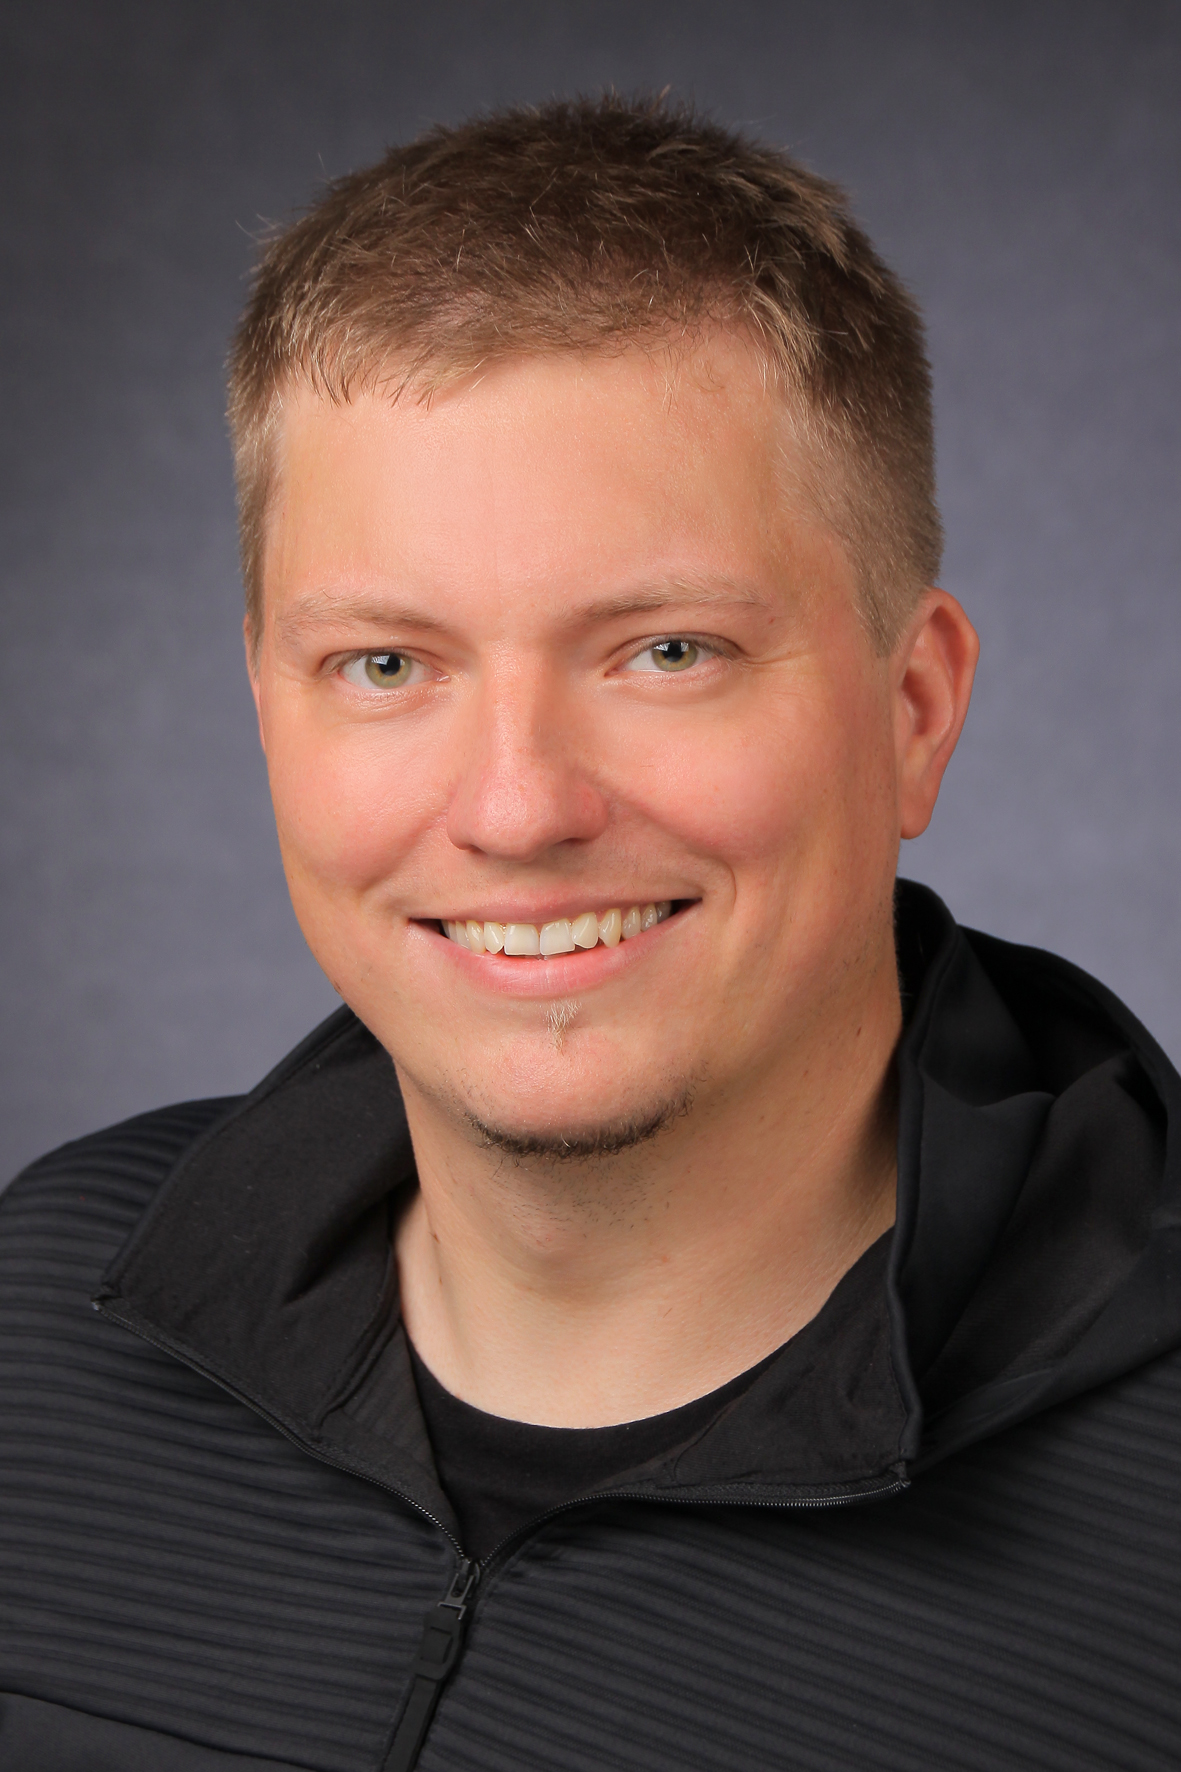
\includegraphics[width=\textwidth]{01-grundlagen/img/dozent_kutscher}
            \end{center}
        \end{column}
        \begin{column}{.8\textwidth}
            \begin{itemize}
                \item \textbf{2012:} Diplom ,,Angewandte Informatik''  an der Uni Duisburg-Essen
                mit Vertiefung ,,Verteilte Systeme und Embedded Systems''

                \item \textbf{2011 -- 2012:} Android-Entwicklung im SKIMS Projekt
                (\Href{https://skims.realmv6.org/})

                \item \textbf{2012 -- aktuell:} IT-Consultant bei EXXETA, Schwerpunkte vor allem
                Web-Entwicklung (Full Stack Development), JavaEE Backend, Angular sowie Integration
                von Backendsystemen wie SAP etc.

                \item \textbf{2016 -- aktuell:} IoT-Projekt SMIGHT (\Href{https://demo.smight-mgt.de}),
                Entwicklung von Microservices mit Node.js und SpringBoot in TypeScript, Java und
                Kotlin, Java OSGI Clients für den Raspberry PI

                \item \textbf{Seit 2018:} Dozent an der DHBW Karlsruhe für
                IoT-Integrationsseminar und Projekt, Verteilte Systeme, Hardwarenahe Programmierung
            \end{itemize}
        \end{column}
    \end{columns}
\end{frame}

%%% Folie
\begin{frame}{Vorstellung: Dennis Schulmeister-Zimolong}
    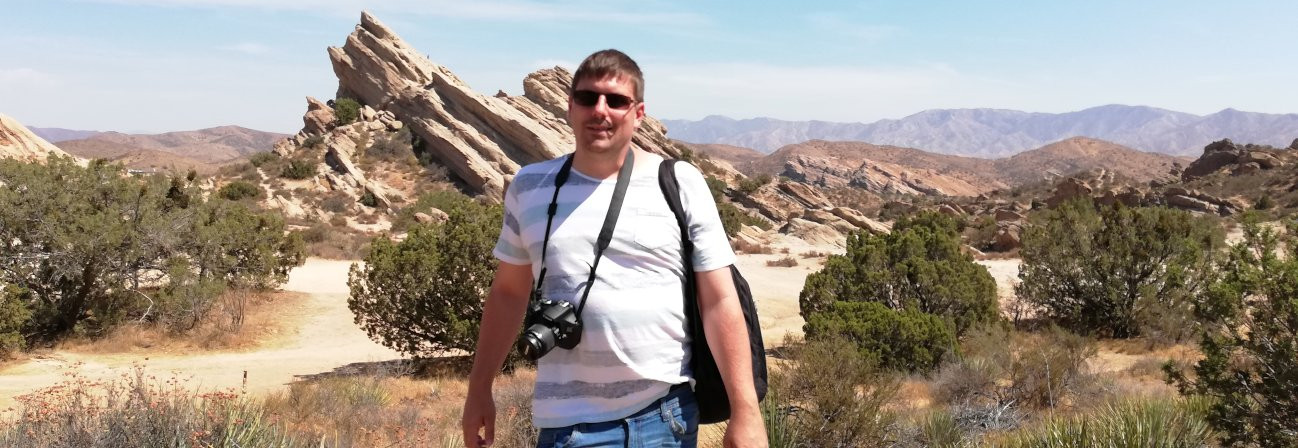
\includegraphics[width=\textwidth]{01-grundlagen/img/dozent_schulmeister}

    \begin{itemize}
        \item Dipl.-Wirtschaftsinformatiker (DH), DHBW Karlsruhe, 2005 – 2008
        \item Produktmanager / Senior Entwickler für SAP Add-Ons, SOA People AG
        \item Seit 2009 nebenberuflicher Dozent an der DHBW Karlsruhe
        \item Seit 1992 begeistert von Computern und deren Programmierung
        \item Keyboarder, Bassist, Sänger und Songwriter in der Freizeit
        \item Seit August 2020 (hoffentlich) der beste Papa der Welt \smiley{}
    \end{itemize}
\end{frame}

%%% Folie
\begin{frame}{Kompetenzziele der Vorlesung}
    \begin{itemize}
        \item \textbf{Fachkompetenz:} Die Studierenden kennen den
        \textcolor{NavyBlue}{technischen Aufbau typischer Devices/Embedded Systems}
        im Kontext des Internet of Things. Sie sind in der Lage, entsprechende Devices
        für einen gegebenen Einsatzzweck auszuwählen und zu programmieren.
        \medskip

        \item \textbf{Methodenkompetenz:} Die Studierenden sind in der Lage
        bei der Programmierung von IoT-Geräten systematisch und methodisch vorzugehen.
        \medskip

        \item \textbf{Personale und soziale Kompetenz:} Die Studierenden verstehen die Herausforderungen
        des IoT für Unternehmen, Politik und Gesellschaft und sind in der Lage, diese kompetent zu diskutieren.
        \medskip

        \item \textbf{Übergreifende Handlungskompetenz:} Die Studierenden können reale betriebliche
        Problemstellungen im Kontext von IoT analysieren, \textcolor{NavyBlue}{Konzepte entwerfen}
        und \textcolor{NavyBlue}{IoT-fähige Geräte programmieren} und im Unternehmenskontext integrieren.
        \medskip
    \end{itemize}
\end{frame}

{
\footnotesize
%%% Folie
\begin{frame}{Inhalte der Vorlesung}
        \begin{columns}
            \begin{column}[T]{.5\textwidth}
                \begin{block}{3. Semester}
                    \medskip

                    \begin{enumerate}
                        \item Grundlagen des Internet of Things
                        \item Hardwaredesign für IoT-Anwendungen
                        \item \textcolor{gray}{Praktische Demonstration}
                        \item \textcolor{gray}{Übungsstunde}
                        \item Einführung in Python
                        \item IoT-Entwicklung mit Python
                        \item \textcolor{gray}{Praktische Demonstration}
                        \item \textcolor{gray}{Übungsstunde}
                        \item \textcolor{gray}{Klausurvorbereitung}
                    \end{enumerate}

                    \medskip
                    \textbf{Prüfungsform:} Klausur
                \end{block}
            \end{column}
            \begin{column}[T]{.5\textwidth}
                \begin{block}{4. Semester}
                    \medskip

                    \begin{enumerate}
                        \item Nutzung analoger und digitaler Bauteile
                        \item Python-Architekturmuster für IoT-Devices
                        \item Datenaustausch und Systemintegration
                        \item Linux-Konfiguration und Deployment
                        \item \textcolor{gray}{Assignment}
                        \item \textcolor{gray}{Assignment}
                        \item \textcolor{gray}{Assignment}
                        \item \textcolor{gray}{Assignment}
                        \item \textcolor{gray}{Assignment}
                    \end{enumerate}

                    \medskip
                    \textbf{Prüfungsform:} Assignment
                \end{block}
            \end{column}
        \end{columns}
\end{frame}
}

%%% Folie
\begin{frame}{Vorausgesetztes Wissen}
    \begin{columns}
        \column{\dimexpr\paperwidth-10pt}
        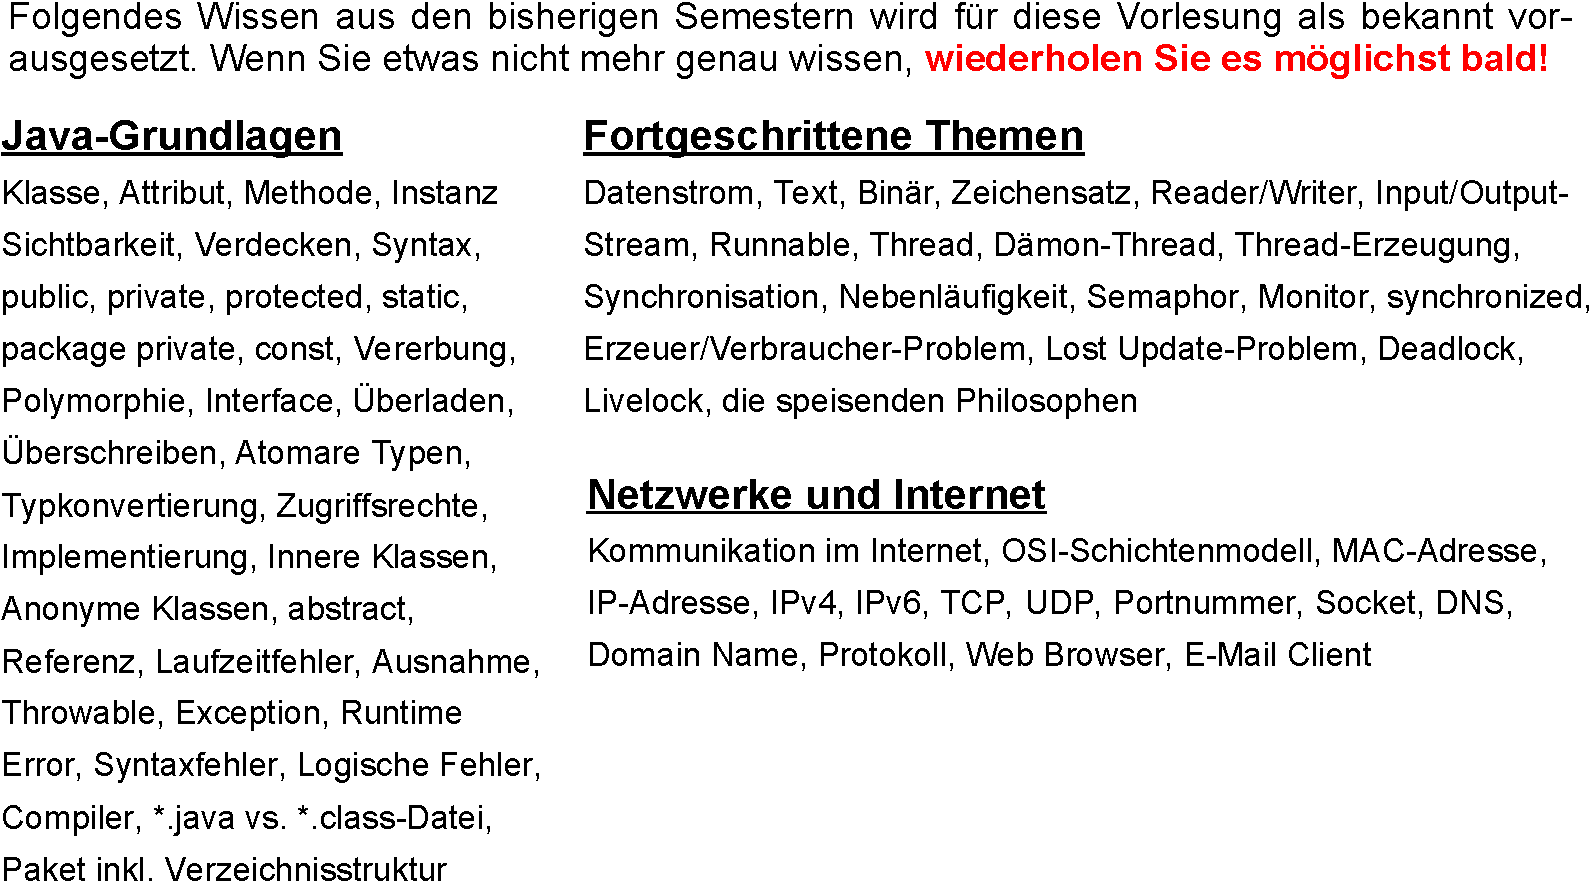
\includegraphics[width=\textwidth]{01-grundlagen/img/vorausgesetztes_wissen}
    \end{columns}
\end{frame}


%%% Folie
\begin{frame}{Benötigte Hard- und Software}
        \begin{columns}
            \begin{column}[T]{.5\textwidth}
                \textbf{Hardware}
                \medskip

                \parbox{\linewidth}{
                    \footnotesize
                    Kann im WWI-Labor für die Dauer des Moduls kostenlos ausgeliehen
                    werden. Rückgabe am Ende des vierten Semesters, da dieselbe
                    Hardware dann direkt für das IoT-Integrationsseminar und Projekt
                    benötigt wird.
                }
                \medskip

                \begin{itemize}
                    \item Raspberry Pi
                    \item Diverse Sensoren und Aktoren
                \end{itemize}
            \end{column}
            \begin{column}[T]{.5\textwidth}
                \textbf{Software}
                \medskip

                \parbox{\linewidth}{
                    \footnotesize
                    Eigentlich nicht viel. Das meiste ist unter Raspbian bereits
                    installiert oder wird von uns im Laufe der Vorlesung ergänzt.
                    Auf Ihrem Laptop benötigen Sie ggf. noch folgende Programme:
                }
                \medskip

                \begin{itemize}
                    \item Visual Studio Code
                    \item OpenSSH / PuTTY
                    \item Optional: Python
                \end{itemize}
            \end{column}
        \end{columns}
\end{frame}

%%% Folie
{
\small
\setlength{\fboxsep}{0pt}

\begin{frame}{Literaturempfehlungen}
    \begin{columns}
        \column[b]{.33\textwidth}
        \fbox{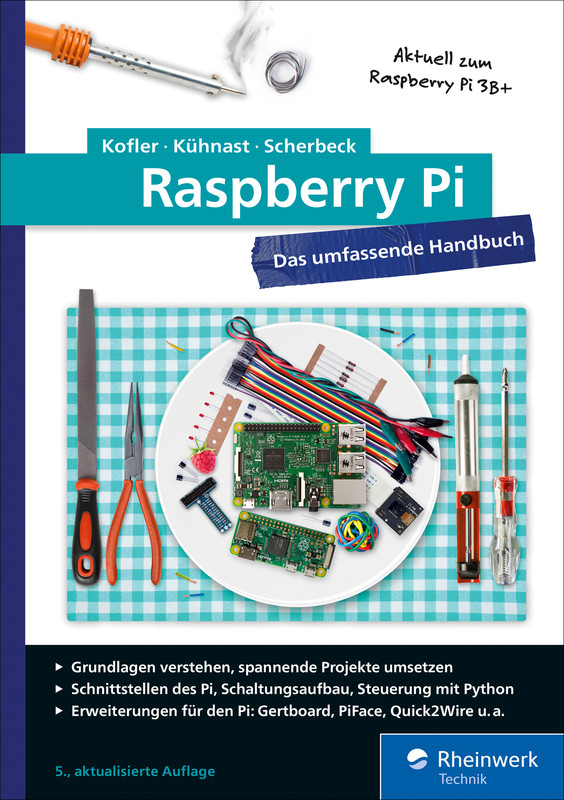
\includegraphics[height=3.8cm]{01-grundlagen/img/buch_raspberrypi}}

        \column[b]{.33\textwidth}
        \fbox{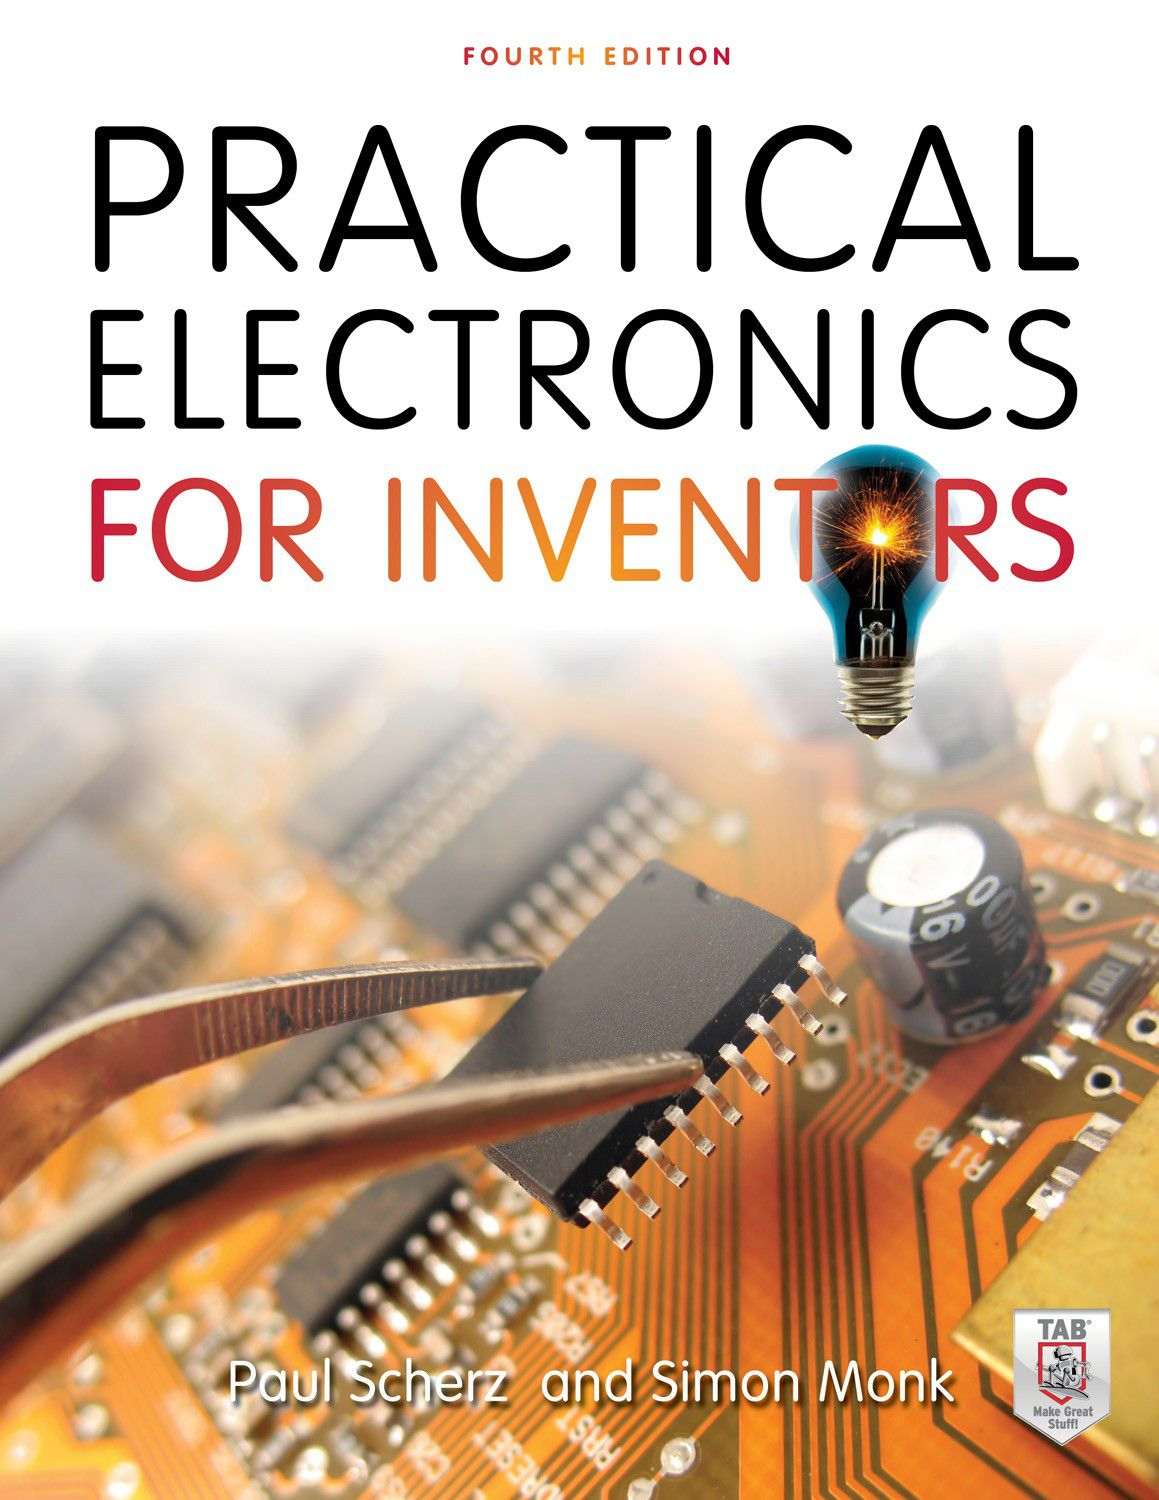
\includegraphics[height=3.8cm]{01-grundlagen/img/buch_practical_electronics}}

        \column[b]{.33\textwidth}
        \fbox{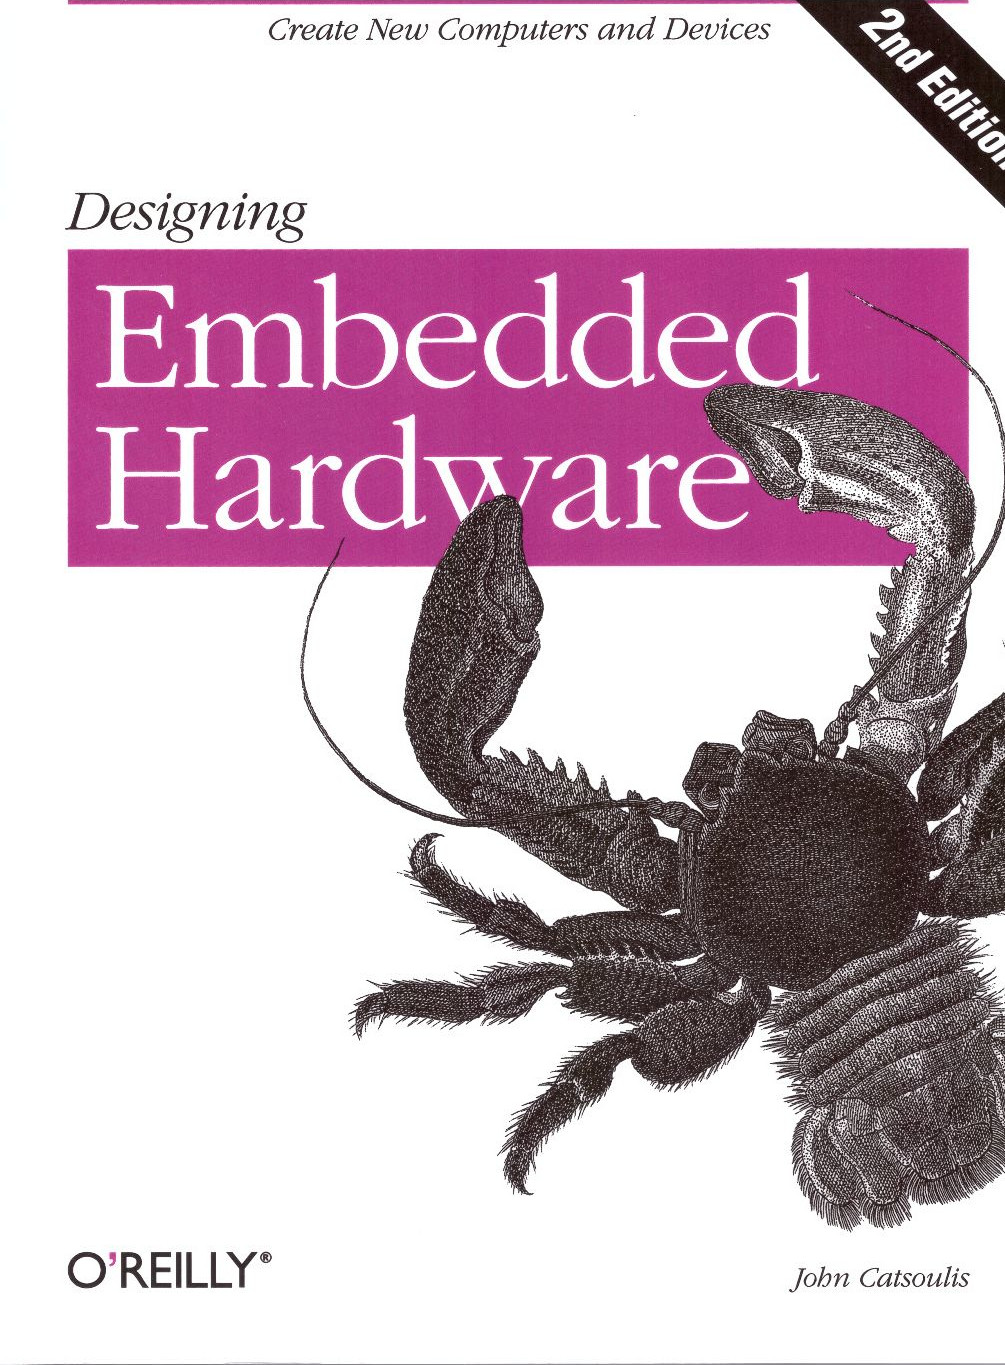
\includegraphics[height=3.8cm]{01-grundlagen/img/buch_embedded_hardware}}
    \end{columns}

    \vskip 0.6cm

    \begin{columns}
        \column[T]{.5\textwidth}
        \textbf{Raspberry Pi: Das umfassende Handbuch für Maker und Tekkies} \\ Rheinwerk Verlag, 2018

        \column[T]{.5\textwidth}
        \textbf{Practical Electronics for Inventors} \\ McGraw-Hill, 2016
    \end{columns}

    \vskip 0.6cm

    \begin{columns}
        \column[T]{0.5\textwidth}
        \textbf{Designing Embedded Hardware} \\ O'Reilly, 2005
    \end{columns}
\end{frame}
}

%%% Folie
\begin{frame}{Lernziele für heute}
    \begin{itemize}
        \item Die Bedeutung des Internet der Dinge in der heutigen Zeit verstehen
        \item Aktuelle IoT-Anwendungsfälle und Geschäftsprozesse erkennen
        \item ,,Internet of Things'' und ,,eingebettete Systeme'' voneinander abgrenzen
        \item Typische Schichten und Komponenten einer IoT-Architektur benennen
        \item Den aktuellen Stand der Technik im historischen Kontext einordnen
        \item Relevante Computerarchitekturen miteinander vergleichen
        \item Die Begriffe ,,Microcontroller'' und ,,System-on-a-Chip'' erklären
        %\item Die Anforderungen an eingebettete Hard- und Software verstehen
    \end{itemize}
\end{frame}

%-------------------------------------------------------------------------------
\section{IoT-Anwendungsfälle}
%-------------------------------------------------------------------------------

%%% Folie
\begin{frame}{Embedded- und IoT-Devices im Alltag}
    \begin{columns}
        \column{\dimexpr\paperwidth-28pt}
        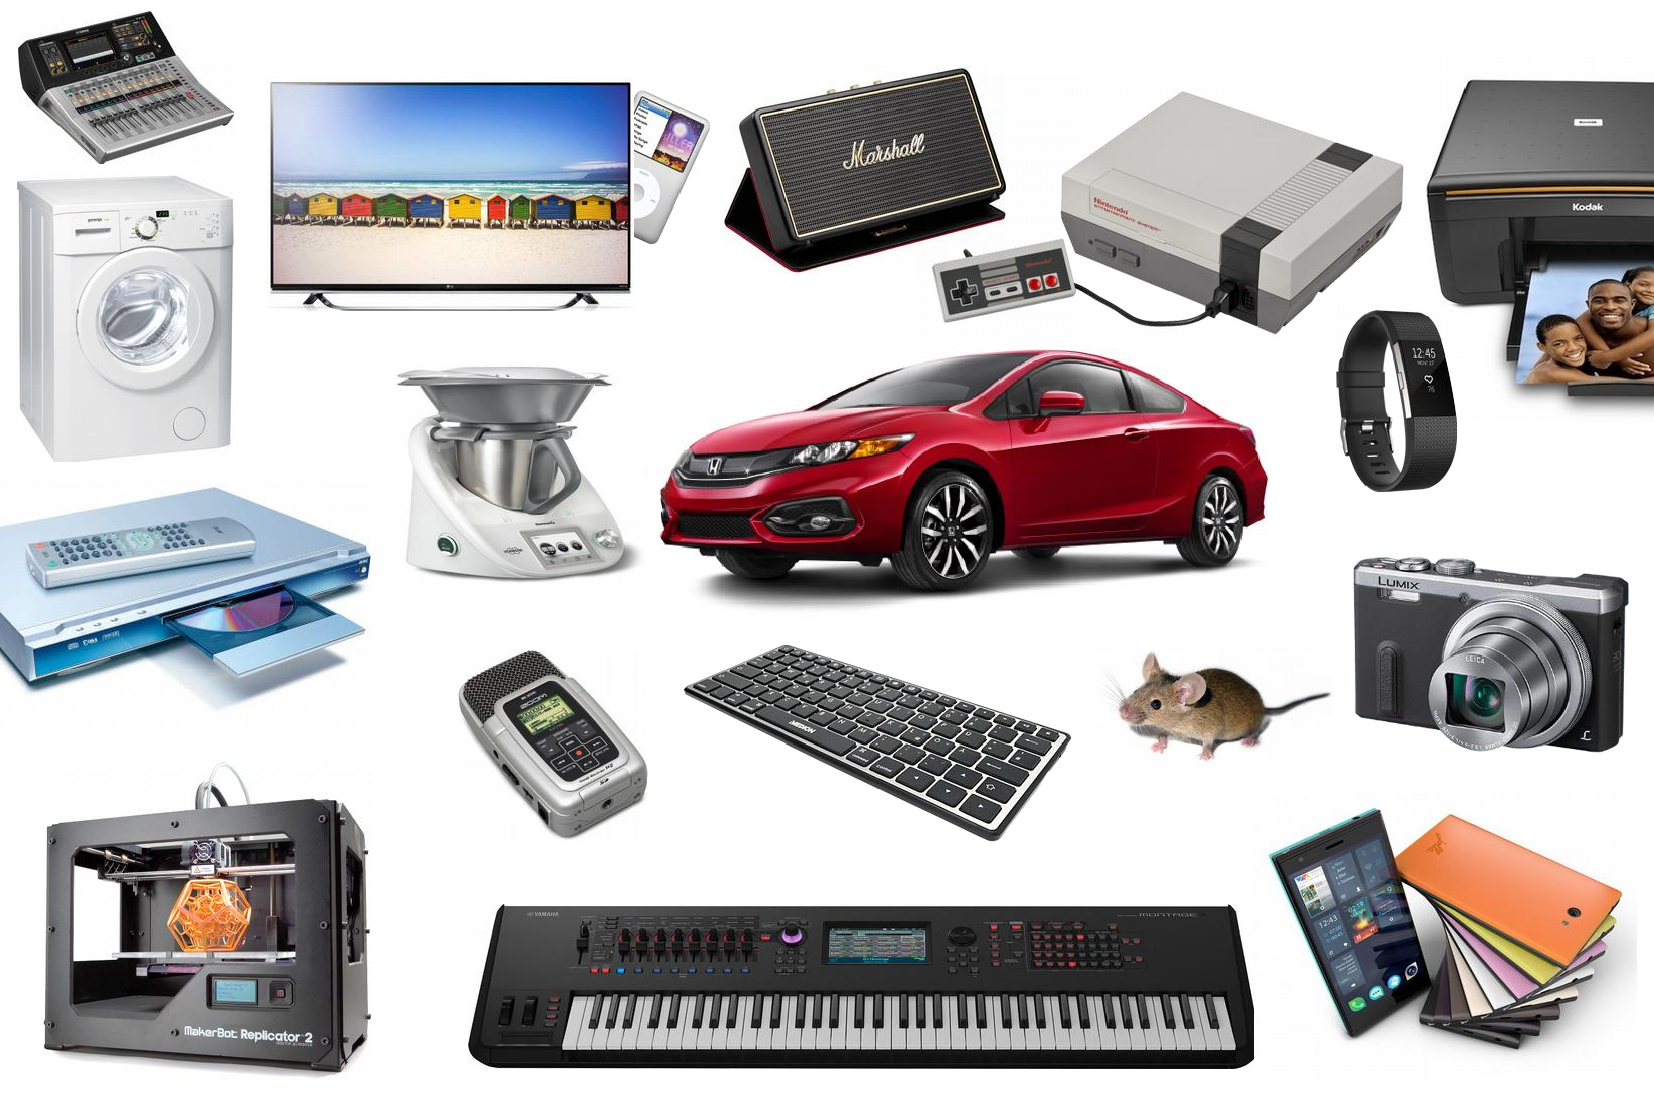
\includegraphics[width=\textwidth]{01-grundlagen/img/embedded_devices}
    \end{columns}
\end{frame}

%%% Folie
\begin{frame}{Embedded/IoT-Devices im Alltag}
    \begin{columns}
        \begin{column}[b]{.5\textwidth}
            \begin{center}
                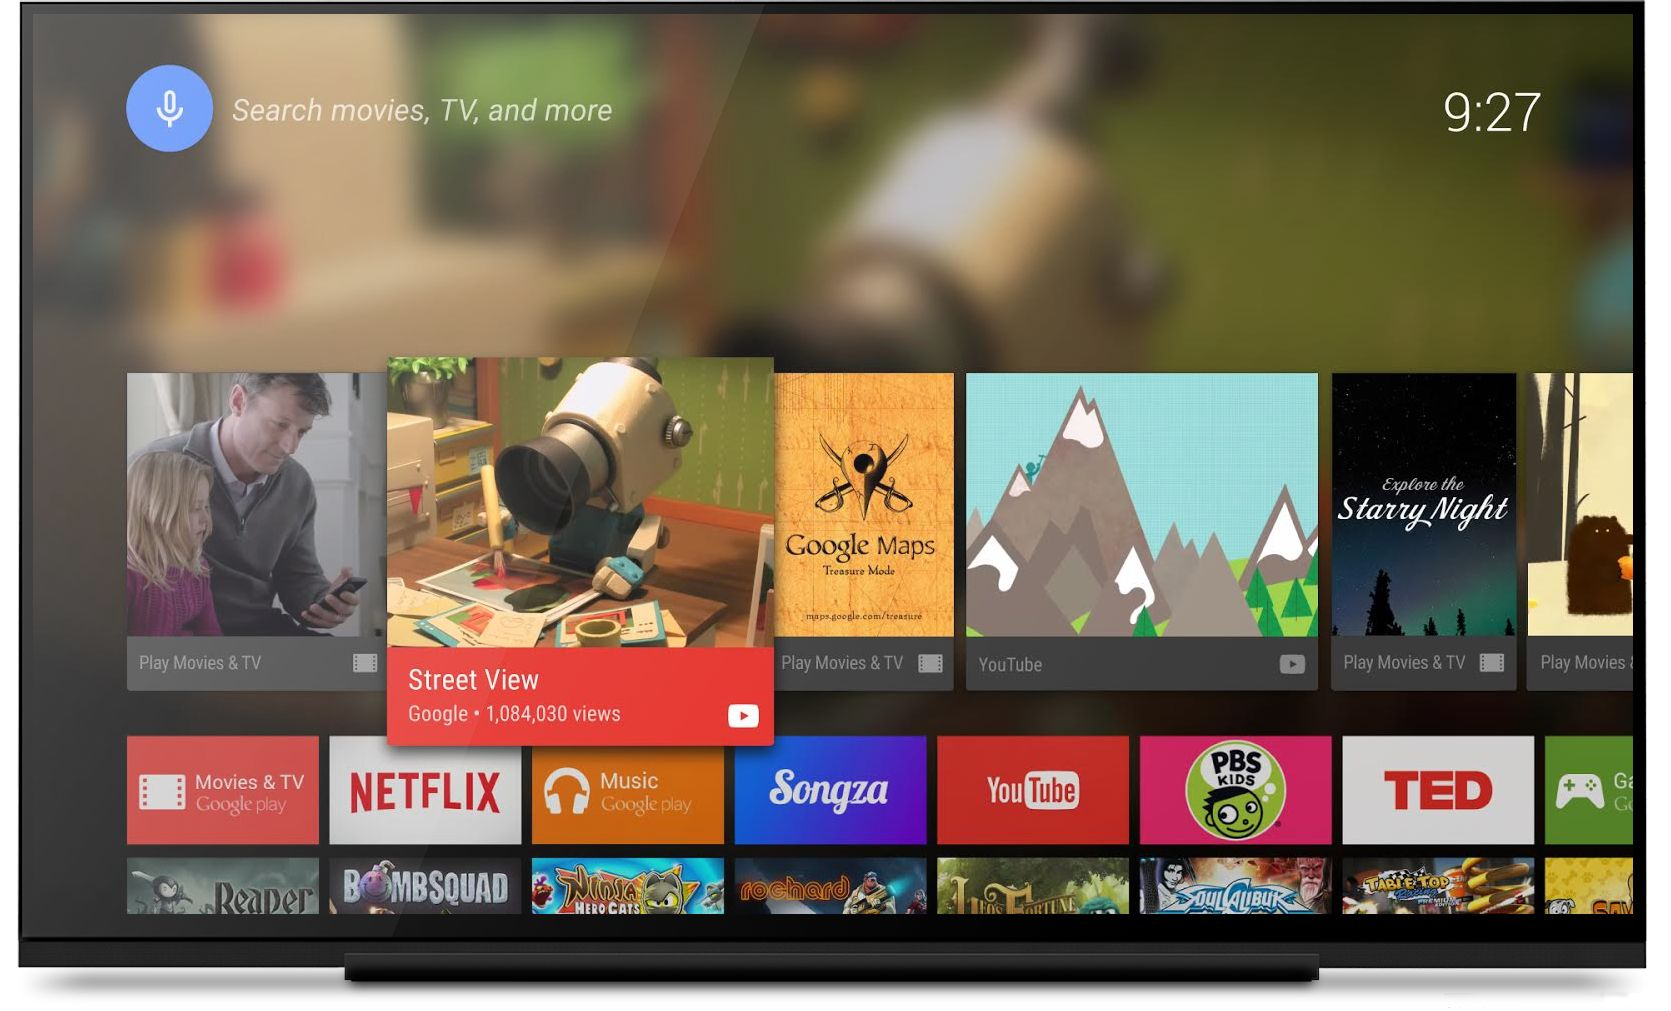
\includegraphics[width=\textwidth]{01-grundlagen/img/android_tv}
            \end{center}
        \end{column}
        \begin{column}[b]{.5\textwidth}
            \begin{center}
                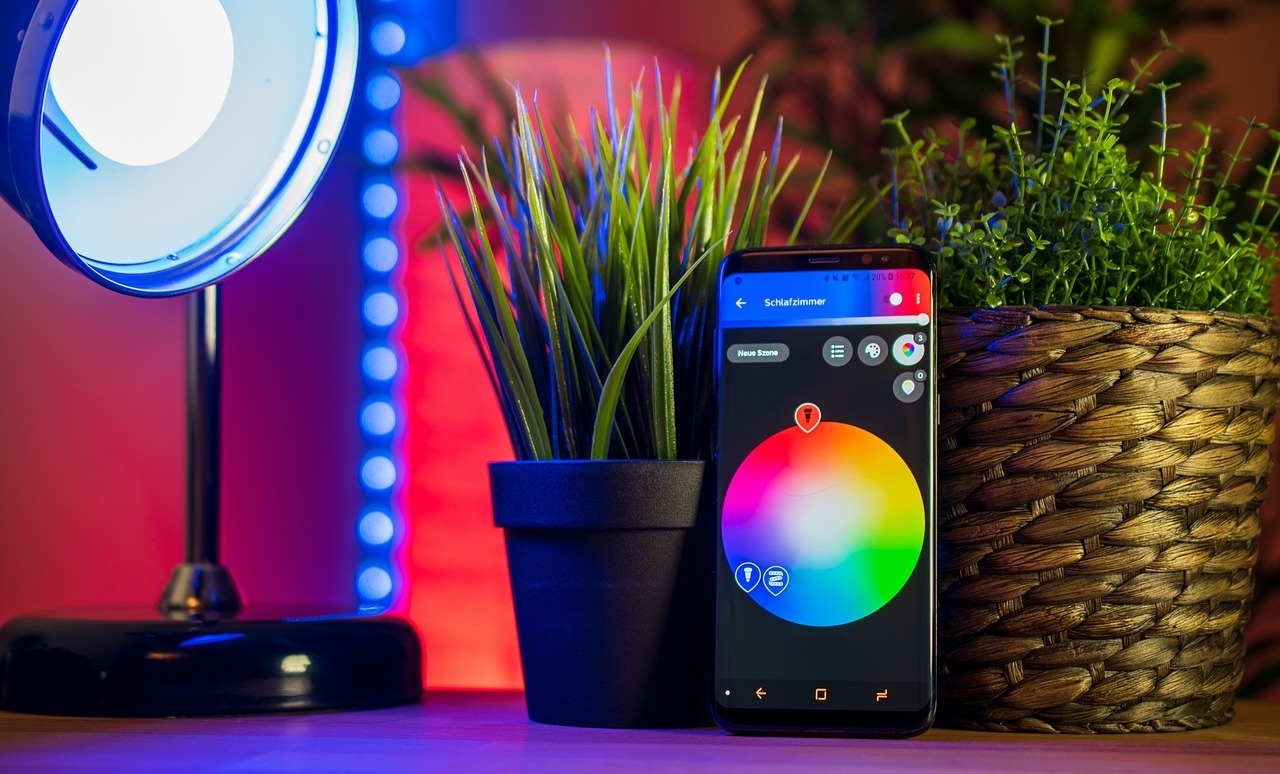
\includegraphics[width=\textwidth]{01-grundlagen/img/smart-home-3779361_1280}
            \end{center}
        \end{column}
    \end{columns}

    \bigskip

    \begin{itemize}
        \item Was bedeutet der Begriff ,,Internet of Things''?
        \item Was macht ein Device zu einem IoT-Device?
        \item Wie unterscheidet es sich von gewöhnlichen Embedded-Devices?
        \item Welche Anwendungsfälle für IoT können Sie sich vorstellen?
    \end{itemize}
\end{frame}

%%% Folie
\begin{frame}{Industrielle IoT-Anwendungsfälle}
    \textbf{Smight -- Smart City Light}
    \hfill
    \Href{https://smight.com/}
    \medskip
    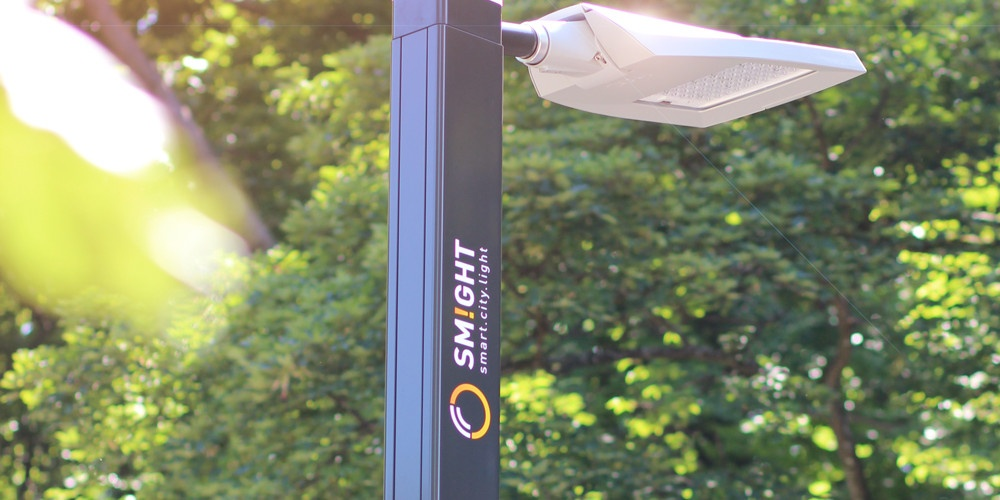
\includegraphics[width=0.49\textwidth]{01-grundlagen/img/smight1}
    \hfill
    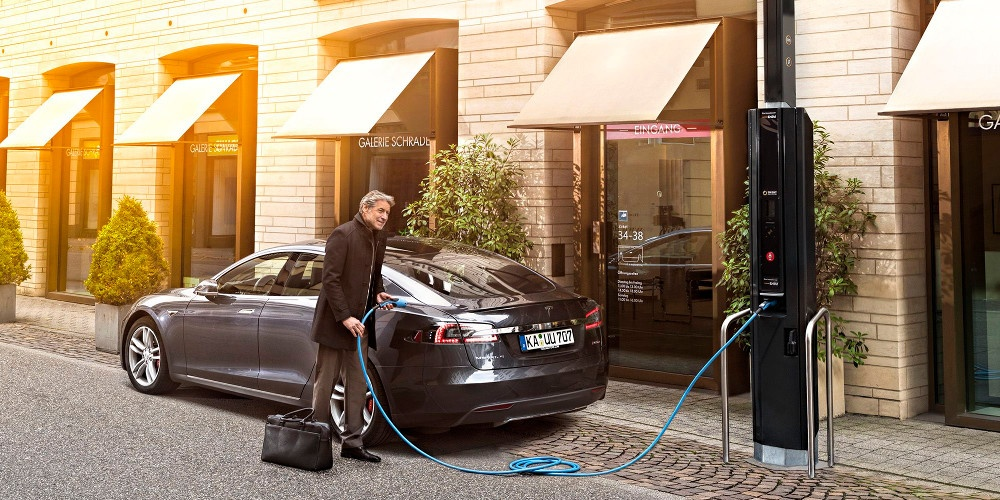
\includegraphics[width=0.49\textwidth]{01-grundlagen/img/smight2}

    \bigskip

    \textbf{Testfeld autonomes Fahren Baden-Württemberg}
    \hfill
    \Href{https://taf-bw.de/}
    \medskip
    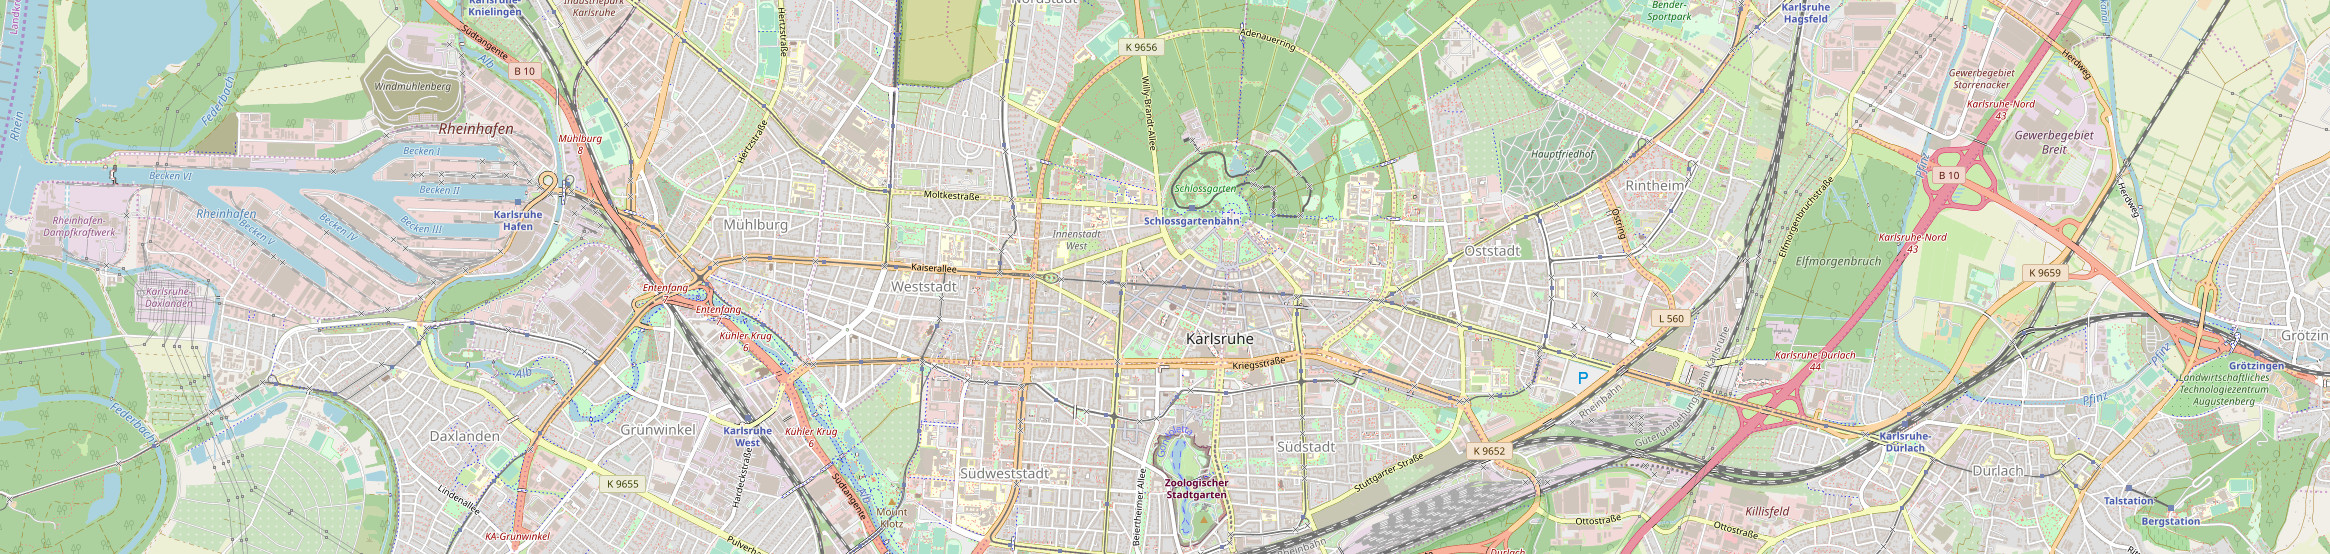
\includegraphics[width=\textwidth]{01-grundlagen/img/karlsruhe}
\end{frame}

%-------------------------------------------------------------------------------
\section{Technische Grundlagen}
%-------------------------------------------------------------------------------

{
\small

%%% Folie
\begin{frame}{Definition ,,Eingebettetes Computersystem''}
    \begin{block}{Definition}
        \parbox{\linewidth}{
            \smallskip

            Eingebettete Systeme sind kleine Mikrocomputer, die innerhalb eines größeren Geräts
            meist unsichtbar verbaut sind, um seine Funktionen zu steuern und überwachen. In vielen
            Fällen geben sie einem Gerät überhaupt erst seine Funktion, ohne dass dies für den
            Anwender offensichtlich ist.
            \smallskip

            Ihre grundsätzliche Architektur ist dieselbe wie bei konventionellen Computern,
            jedoch verfügen sie über weitaus weniger, genau auf den Anwendungsfall zugeschnittene
            Ressourcen bei minimalen Kosten, Platzbedarf und Energieverbrauch. Der Leitgedanke
            hierbei lautet ,,so viel wie gerade nötig, so wenig wie absolut möglich''.
            Eingebettete Systeme sind meist in sich geschlossene Systeme mit deterministischem
            Systemverhalten, die rund um die Uhr laufen und exakt eine Aufgabe erfüllen.
        }
    \end{block}

    \begin{block}{Beispiele}
        \begin{columns}[onlytextwidth]
            \column[b]{.2\textwidth}
            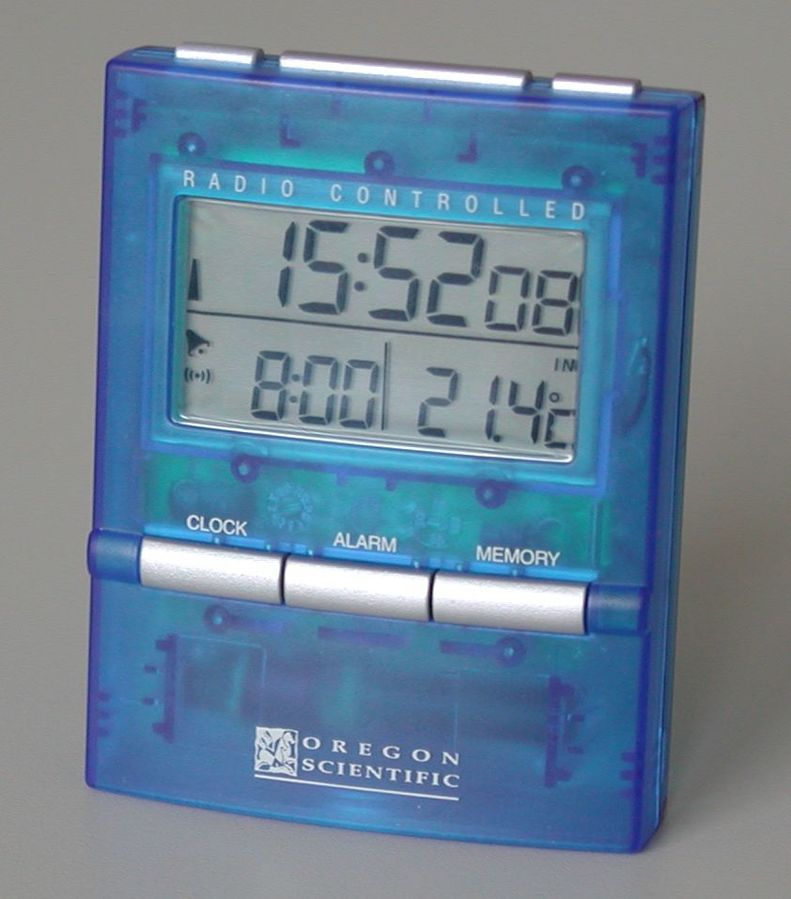
\includegraphics[width=\textwidth]{01-grundlagen/img/funkwecker}

            \column[b]{.2\textwidth}
            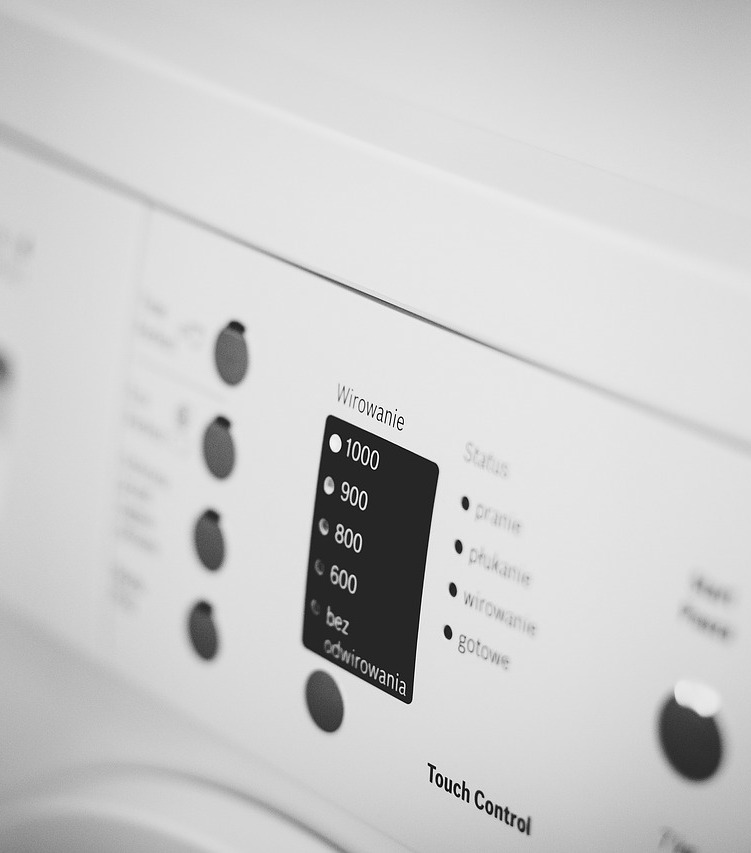
\includegraphics[width=\textwidth]{01-grundlagen/img/washing-machine-2617514_1280}

            \column[b]{.2\textwidth}
            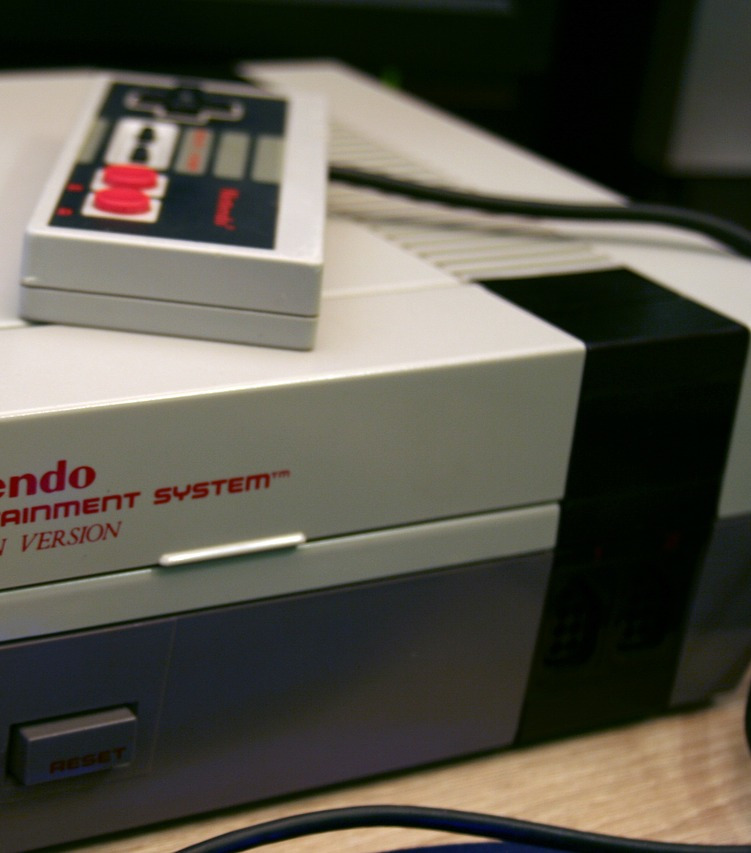
\includegraphics[width=\textwidth]{01-grundlagen/img/nes-2649705_1280}

            \column[b]{.2\textwidth}
            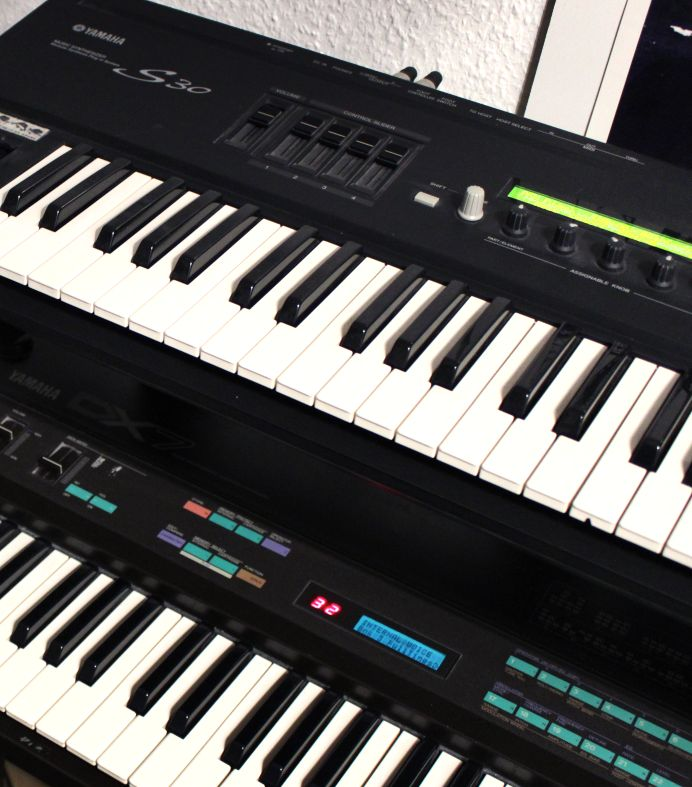
\includegraphics[width=\textwidth]{01-grundlagen/img/keyboards}

            \column[b]{.2\textwidth}
            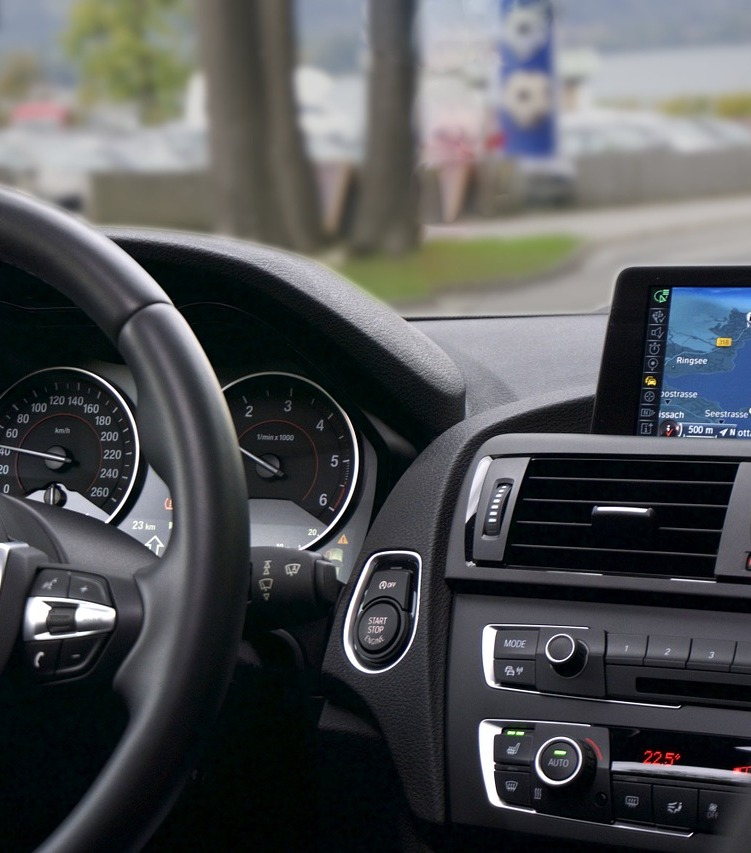
\includegraphics[width=\textwidth]{01-grundlagen/img/car-1281640_1280}
        \end{columns}
    \end{block}
\end{frame}

%%% Folie
\begin{frame}{Definition ,,Internet of Things''}
    \begin{block}{Definition}
        \parbox{\linewidth}{
            \smallskip

            IoT-Devices sind eine Teilmenge eingebetteter Systeme größerer Leistungsklasse mit
            permanenter Internetverbindung. Die ursprüngliche Definition aus dem Jahr 1999
            sah die eindeutige, maschinenlesbare Identifikation physischer Objekte anhand von
            RFID-Tags vor. Heute versteht man darunter an einem physischen Objekt angebrachte,
            direkt mit dem Internet verbundene und über ihre IP-Adresse identifizierte Kleinstcomputer,
            da diese inzwischen auf wenigen Quadratzentimetern Platz finden.
            \smallskip

            Im erweiterten Sinne zählen zum ,,Internet of Things'' heute auch Infrastruktur, Cloud-
            und Backendservices, über welche die Devices miteinander verbunden, verwaltet, gesteuert
            und überwacht werden können.
        }
    \end{block}

    \medskip
    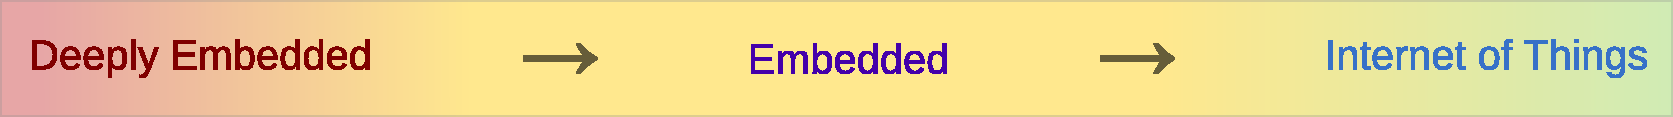
\includegraphics[width=\textwidth]{01-grundlagen/img/embedded_typen}

    \begin{block}{Beispiele}
        \begin{columns}[onlytextwidth]
            \column[b]{.33\textwidth}
            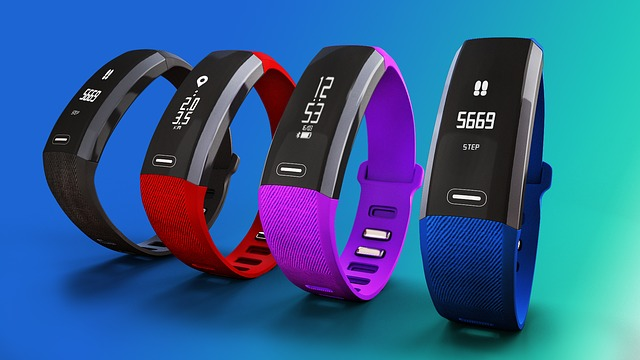
\includegraphics[width=\textwidth]{01-grundlagen/img/heart-rate-monitoring-device-1903997_640}

            \column[b]{.33\textwidth}
            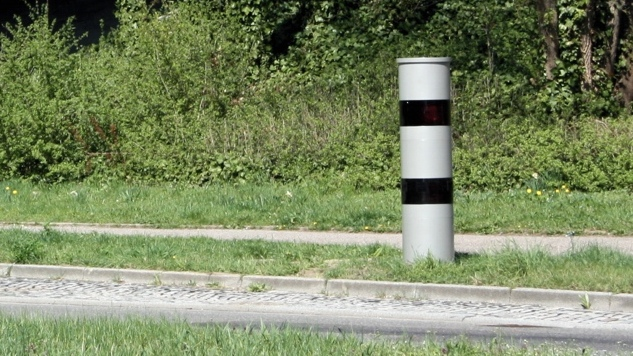
\includegraphics[width=\textwidth]{01-grundlagen/img/blitzer_pulverhausstrasse}

            \column[b]{.33\textwidth}
            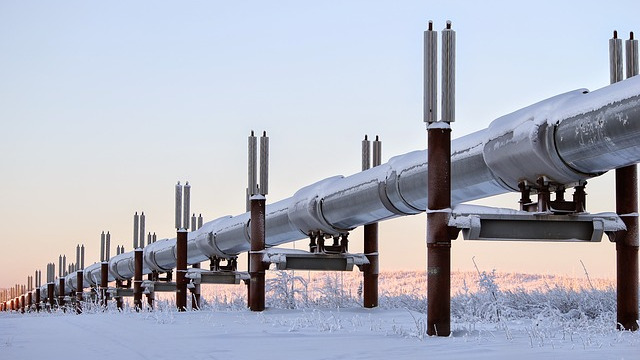
\includegraphics[width=\textwidth]{01-grundlagen/img/winter-681175_640}
        \end{columns}
    \end{block}
\end{frame}
}

%%% Folie
{
\setbeamertemplate{background canvas}{
    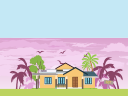
\includegraphics[height=\paperheight, width=\paperwidth]{01-grundlagen/img/themengebiete1}
}

\begin{frame}[fragile]{IoT -- Ein Haus mit tiefem Keller}
    \only<beamer:2|handout:0>{
        \transdissolve

        \begin{tikzpicture}[remember picture,overlay]
            \node at (5.4cm,0.28cm){
                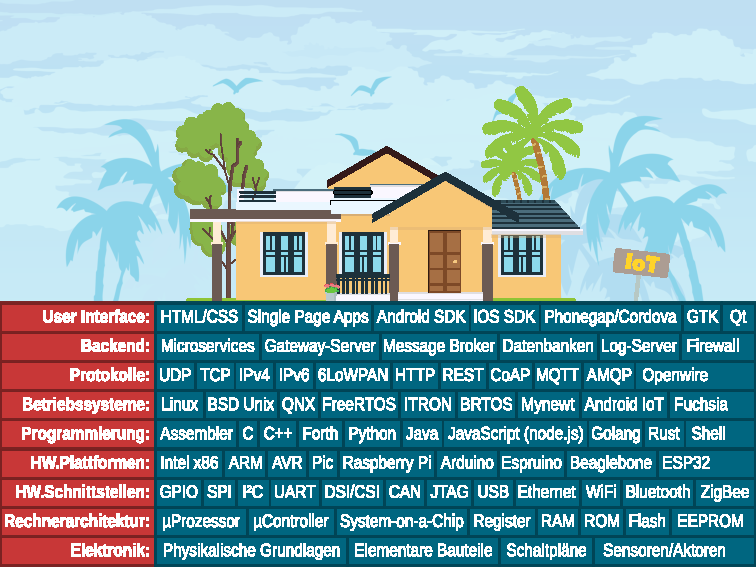
\includegraphics[height=\paperheight, width=\paperwidth]{01-grundlagen/img/themengebiete2}
            };
        \end{tikzpicture}
    }

    \only<beamer:3|handout:0>{
        \transdissolve

        \begin{tikzpicture}[remember picture,overlay]
            \node at (5.4cm,0.28cm){
                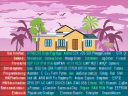
\includegraphics[height=\paperheight, width=\paperwidth]{01-grundlagen/img/themengebiete3}
            };
        \end{tikzpicture}
    }

    \only<beamer:4|handout:0>{
        \transdissolve

        \begin{tikzpicture}[remember picture,overlay]
            \node at (5.4cm,0.28cm){
                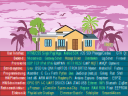
\includegraphics[height=\paperheight, width=\paperwidth]{01-grundlagen/img/themengebiete4}
            };
        \end{tikzpicture}
    }
\end{frame}
}

{
\setbeamertemplate{background canvas}{
    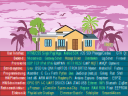
\includegraphics[height=\paperheight, width=\paperwidth]{01-grundlagen/img/themengebiete4}
}

\begin{frame}<handout>[plain]
\end{frame}
}

%%% Folie
\begin{frame}{Beispiel einer typischen IoT-Architektur}
    \begin{columns}
        \column{\dimexpr\paperwidth-10pt}
        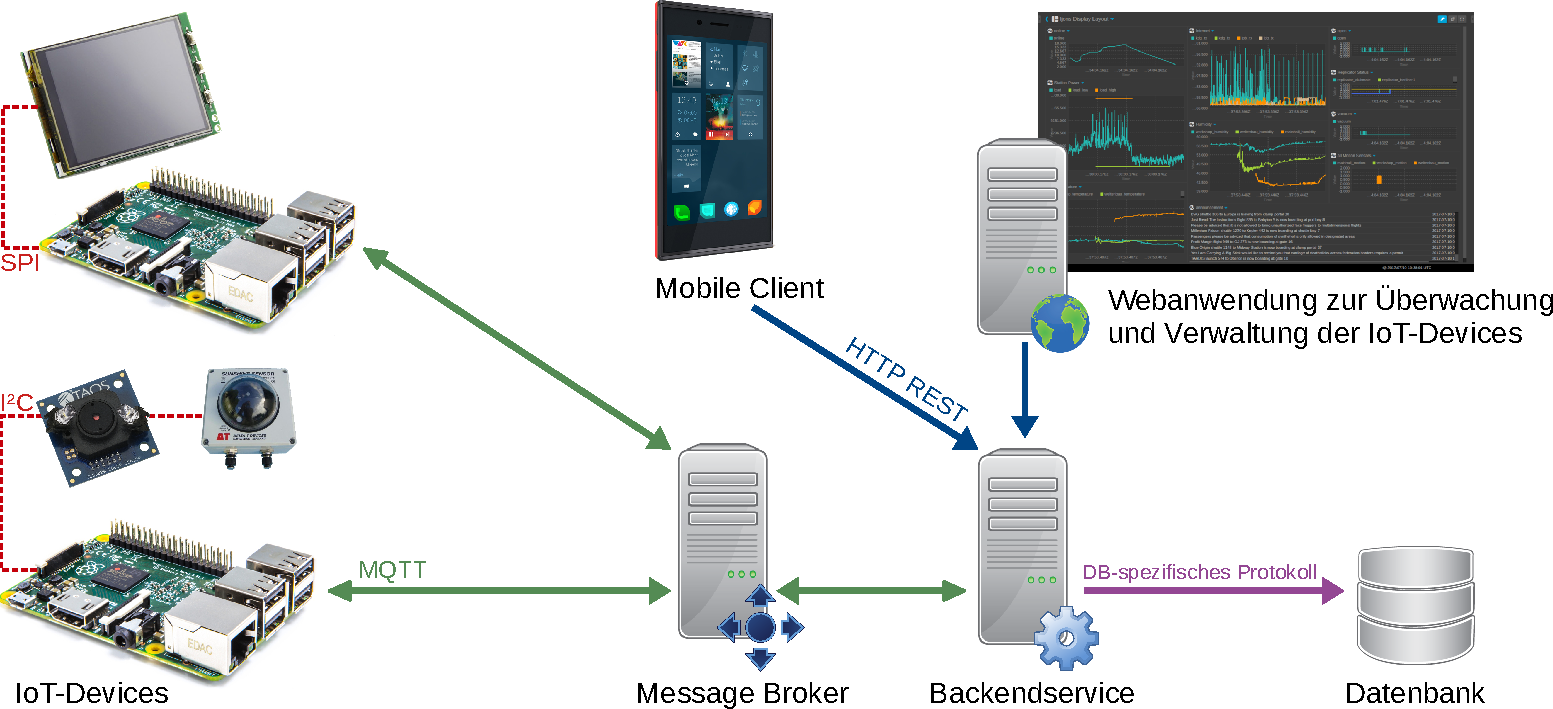
\includegraphics[width=\textwidth]{01-grundlagen/img/architektur_beispiel}
    \end{columns}
\end{frame}

%-------------------------------------------------------------------------------
\section{Eingebettete Rechnerarchitekturen}
%-------------------------------------------------------------------------------

%%% Folie
\begin{frame}[allowframebreaks]{Eine kleine Computer-Geschichte}
    \begin{columns}
        \column{\dimexpr\paperwidth-10pt}
        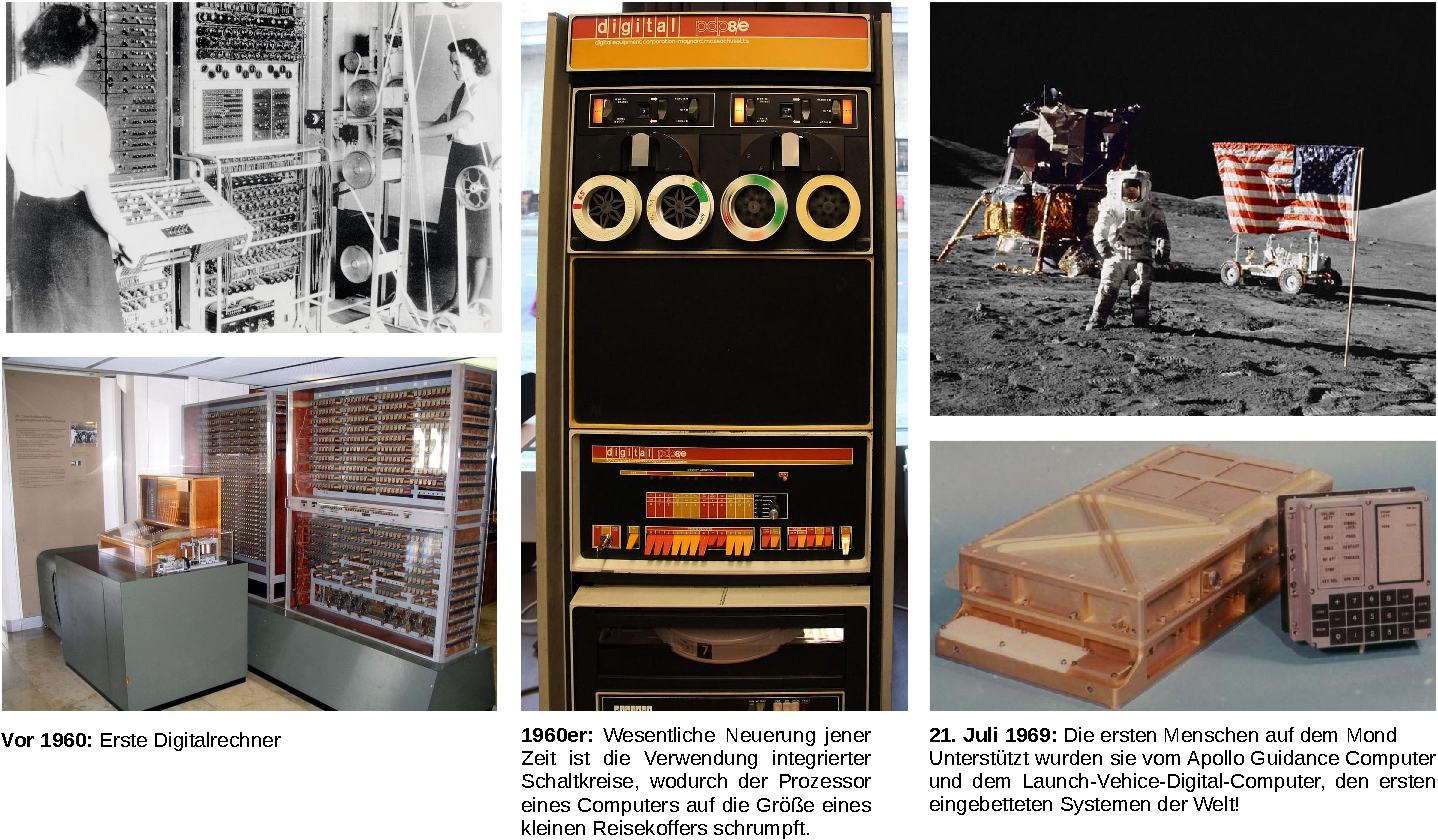
\includegraphics[width=\textwidth]{01-grundlagen/img/geschichte1}
    \end{columns}

    \begin{columns}
        \column{\dimexpr\paperwidth-10pt}
        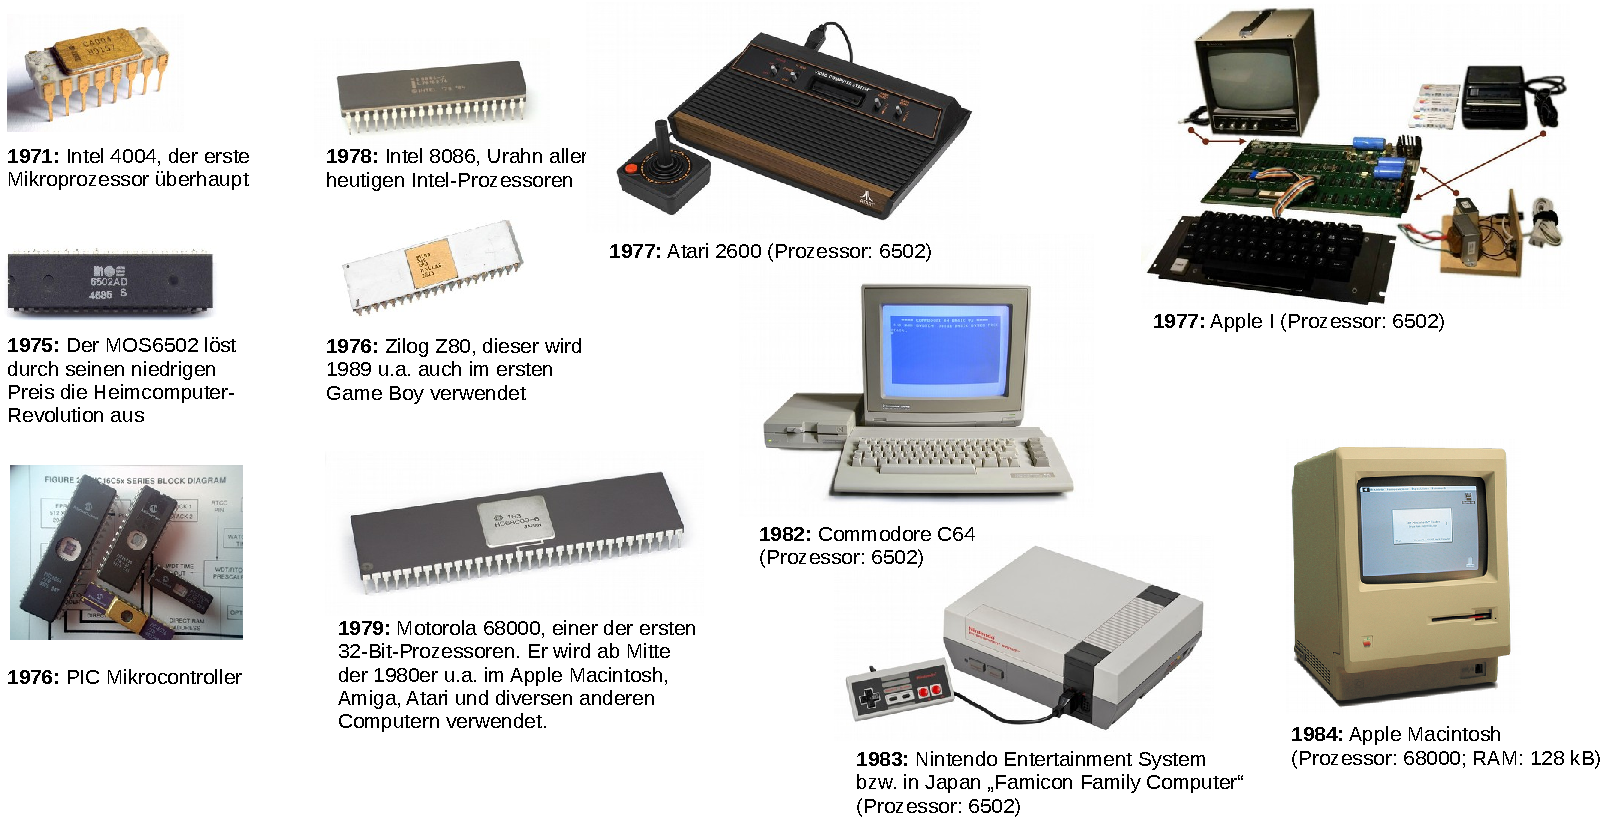
\includegraphics[width=\textwidth]{01-grundlagen/img/geschichte2}
    \end{columns}

    \begin{columns}
        \column{\dimexpr\paperwidth-10pt}
        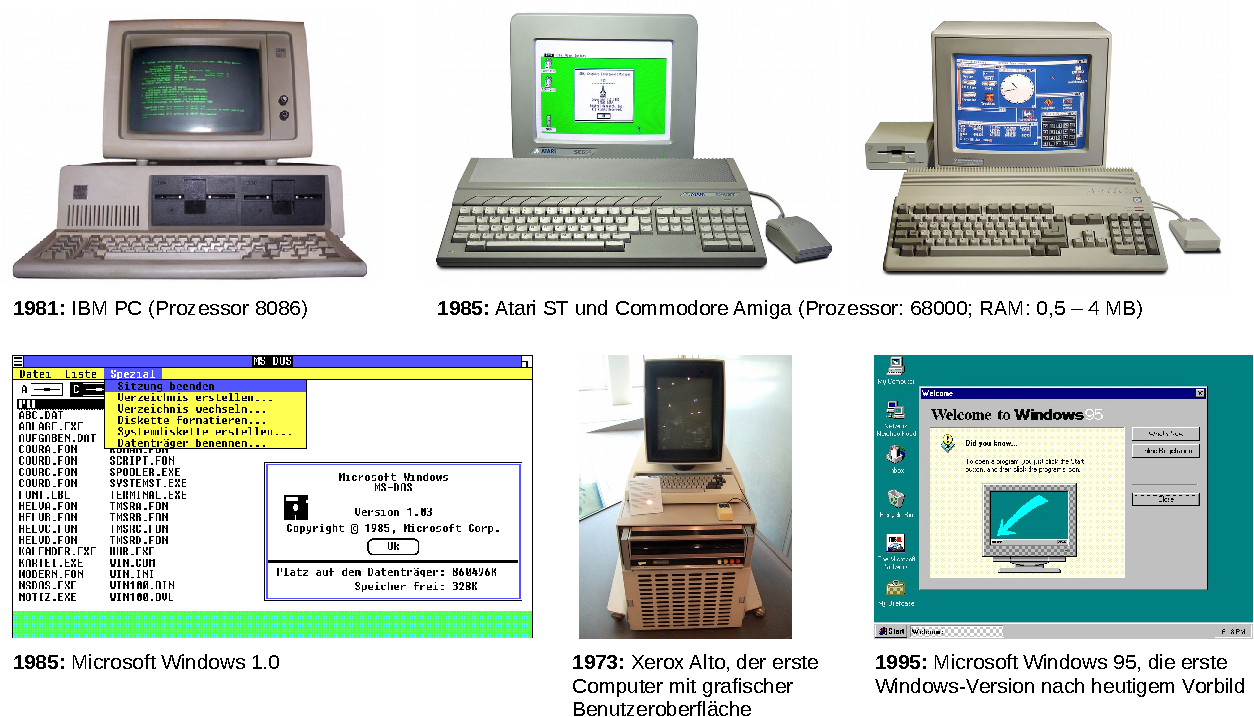
\includegraphics[width=\textwidth]{01-grundlagen/img/geschichte3}
    \end{columns}

    \begin{columns}
        \column{\dimexpr\paperwidth-10pt}
        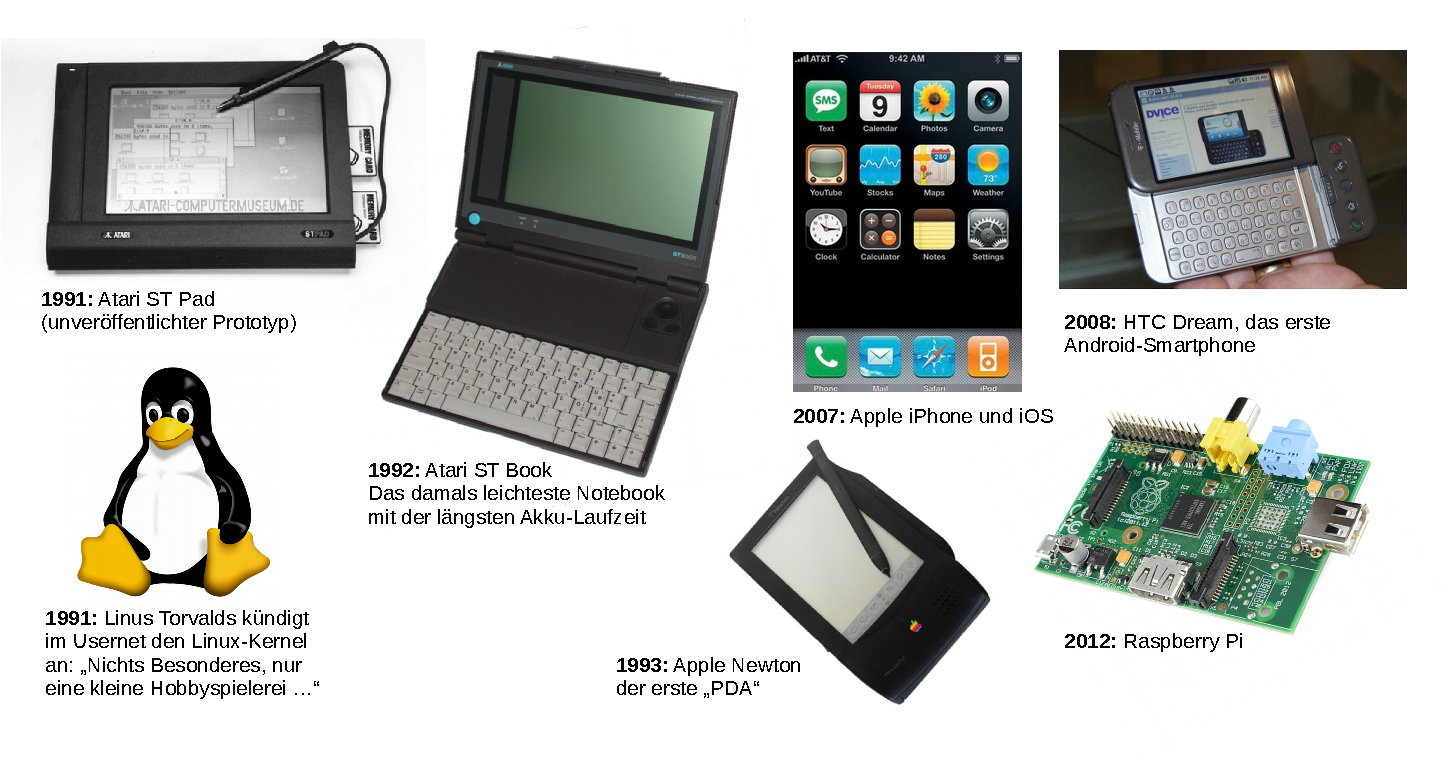
\includegraphics[width=\textwidth]{01-grundlagen/img/geschichte4}
    \end{columns}
\end{frame}

%%% Folie
\begin{frame}{Die Moral der Geschichte}
    \parbox{\linewidth}{
        \footnotesize

        Der Wunsch, einen Computer zum \textbf{Messen, Steuern und Regeln}
        physikalischer Vorgänge zu nutzen ist fast so alt wie der Computer
        selbst. Die Miniaturisierung der ersten Computer führt bereits früh
        zur Entwicklung eingebetteter Systeme oder der Anpassung vorhandener
        Computersysteme an eingebettete Anwendungsfälle.

        \medskip

        In diesem Sinne hat der Hypebegriff \textbf{\glqq{}Industrie 4.0\grqq{}}
        zwar seine Berechtigung, ist aber nicht in allen Punkten so neuartig,
        wie es einem Glauben gemacht werden soll. (Relativ) neu ist aber, dass
        wir heute zwei Möglichkeiten haben, eingebettete (IoT-)Anwendungen zu
        realisieren:
    }

    \bigskip

    \begin{columns}
        \begin{column}[b]{.5\textwidth}
            \begin{block}{Projektentwicklung}
                \medskip
                %\begin{center}
                    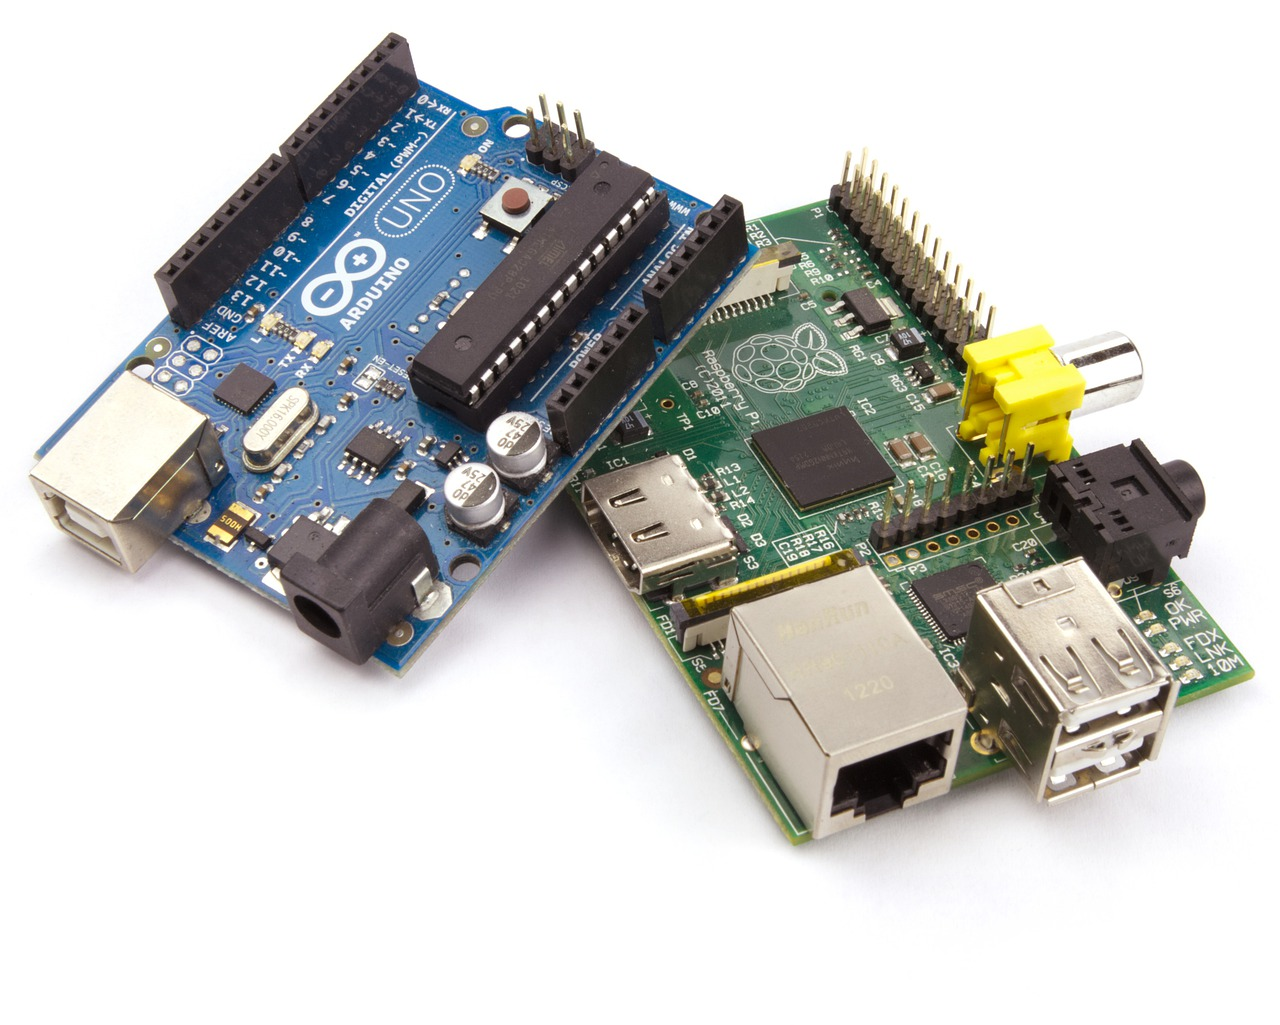
\includegraphics[width=.4\textwidth]{01-grundlagen/img/sbc-boards}
                %\end{center}

                \medskip
                \parbox{\linewidth}{
                    \footnotesize
                    \textbf{Sehr hohe Integrationstiefe:}
                    Verwendung günstiger Single Board Computer als Komplettsystem
                    inkl. Ökosystem für Programmiersprachen und Hardware-Erweiterungen.
                }
            \end{block}
        \end{column}

        \begin{column}[b]{.5\textwidth}
            \begin{block}{Produktentwicklung}
                \medskip
                %\begin{center}
                    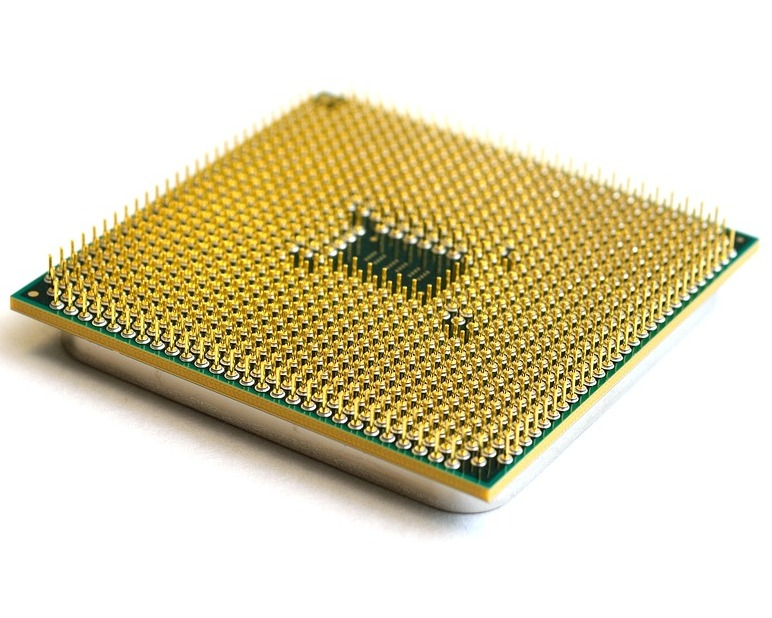
\includegraphics[width=.4\textwidth]{01-grundlagen/img/microchip}
                %\end{center}

                \medskip

                \parbox{\linewidth}{
                \footnotesize
                    \textbf{Mittlere Integrationstiefe}:
                    Eigenentwicklung eingebetteter Computersysteme auf Basis diskreter
                    Bausteine für Microcontroller, Flash-Speicher, RAM, I/O, …
                }
            \end{block}
        \end{column}
    \end{columns}
\end{frame}


%%% Folie
{
    \setbeamertemplate{background canvas}{
        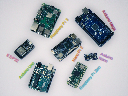
\includegraphics[height=\paperheight, width=\paperwidth]{01-grundlagen/img/sbc_auswahl}
    }

    \begin{frame}[plain]
    \end{frame}
}

%%% Folie
\begin{frame}{Minimale Grundkomponenten eines Computers}
    \begin{center}
        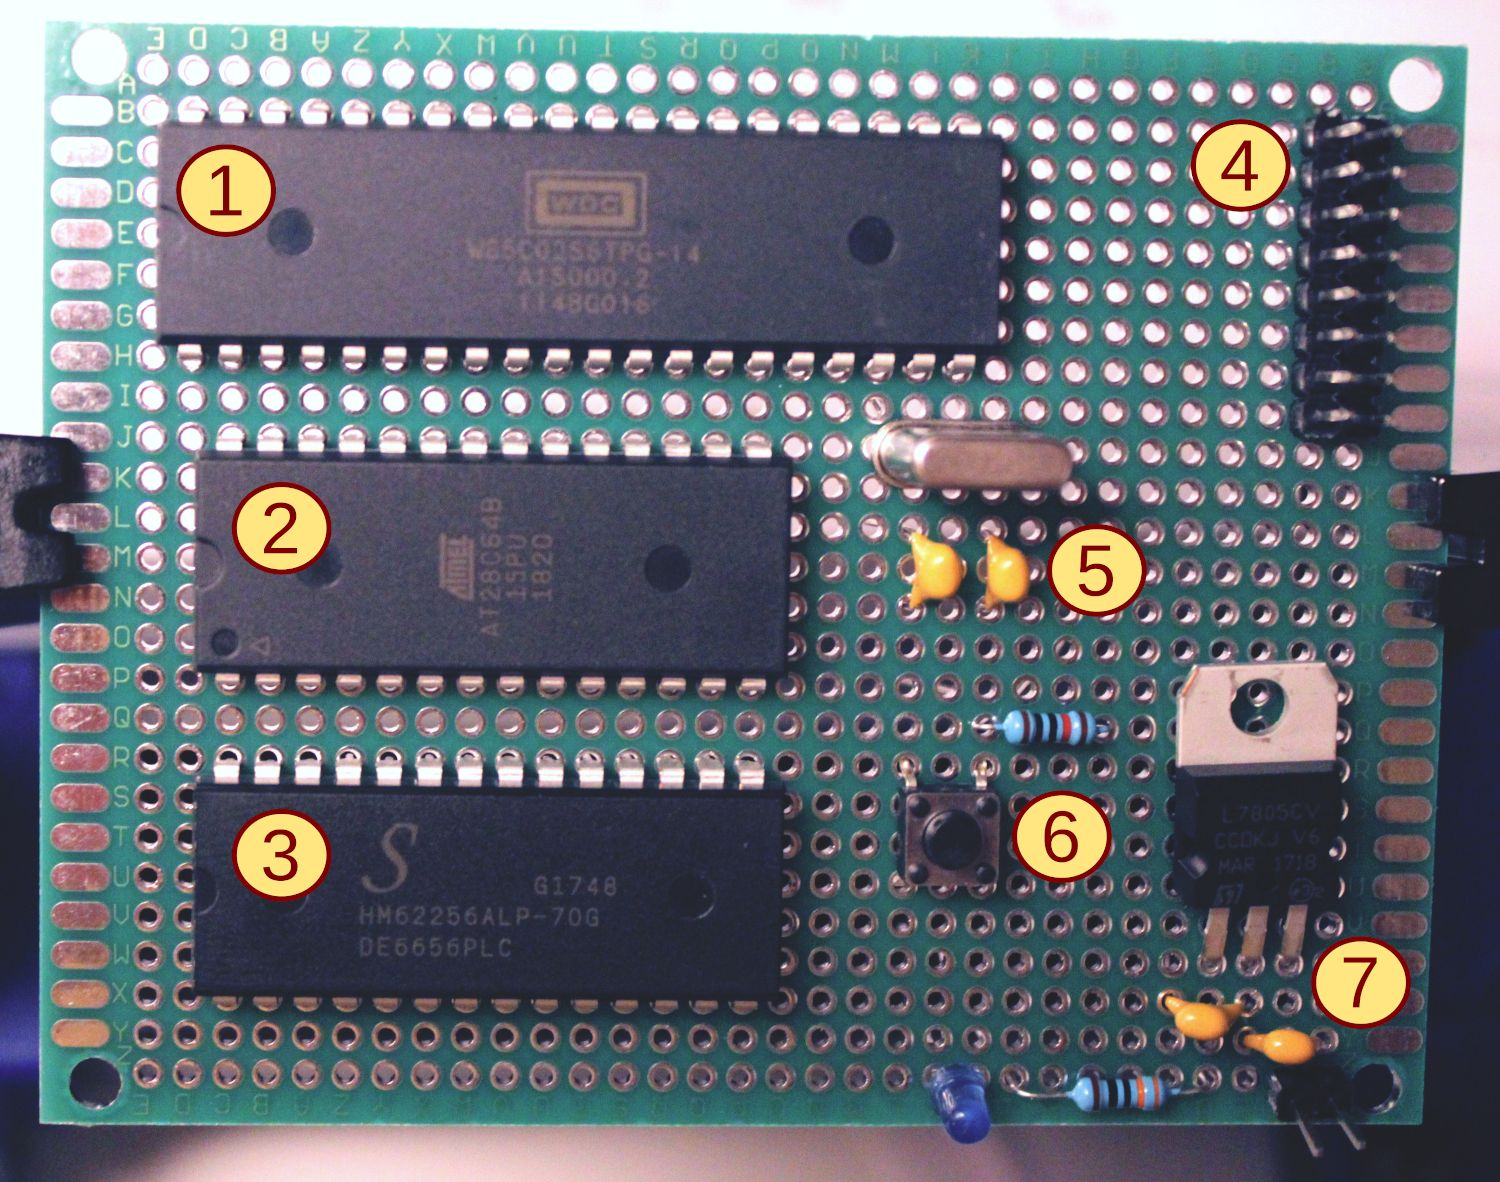
\includegraphics[height=0.5\textheight]{01-grundlagen/img/sbc_microprozessor2_klein}
    \end{center}

    \medskip

    \begin{columns}
        \begin{column}[T]{.5\textwidth}
            \textbf{Digitale Bausteine}
            \begin{enumerate}
                \item Mikroprozessor
                \item Programmspeicher
                \item Hauptspeicher
                \item I/O-Ports
            \end{enumerate}
        \end{column}
        \begin{column}[T]{.5\textwidth}
            \textbf{Hilfsschaltungen}
            \begin{enumerate}
                \setcounter{enumi}{4}
                \item Taktgeber
                \item Resetschalter
                \item Stromversorgung
                \item Adressdekodierung
            \end{enumerate}
        \end{column}
    \end{columns}
\end{frame}

%%% Folie
{
\footnotesize

\begin{frame}{Mikroprozessoren für eingebettete Systeme}
    \begin{columns}
        \column{.2\textwidth}
        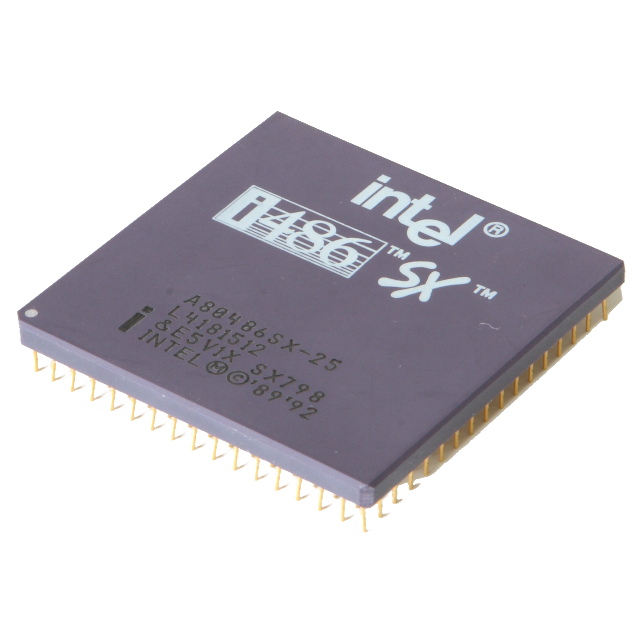
\includegraphics[width=.9\linewidth]{01-grundlagen/img/intel486}

        \column{.8\textwidth}
        \begin{block}{Diskreter Hauptprozessor}
            \parbox{\linewidth}{
                \smallskip

                Bildet das Herzstück eines jeden Computers bzw. stellt den Computer
                im engeren Sinne dar, basierend auf dem Prinzip
                \textbf{Eingabe-Verarbeitung-Ausgabe}. Kommuniziert daher über eine
                \textbf{Speicherschnittstelle} bestehend aus Adress-, Daten- und Steuerleitungen
                mit externen Speicher- und I/O-Bausteinen.
            }

            \smallskip

            \textbf{Beispiele}: Intel 8051, MOS 6502, Motorola 68000, …
        \end{block}
    \end{columns}

    \begin{columns}
        \column{.2\textwidth}
        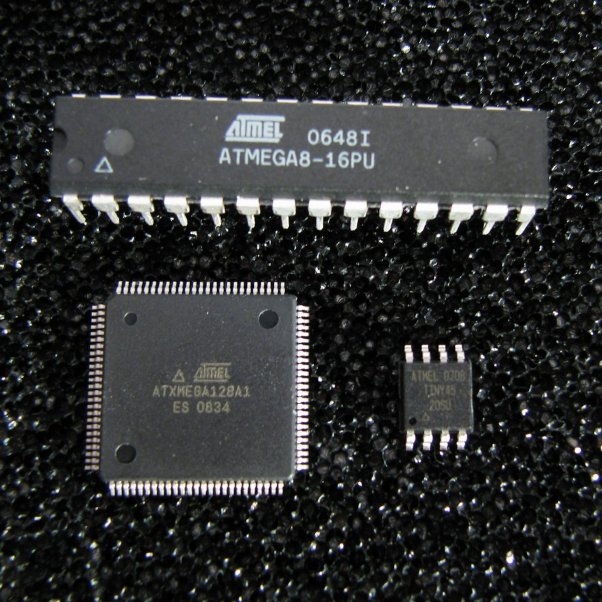
\includegraphics[width=.9\linewidth]{01-grundlagen/img/AVR-ATmega}

        \column{.8\textwidth}
        \begin{block}{Microcontroller}
            \parbox{\linewidth}{
                \smallskip

                Integriert eine einfache CPU (oftmals mit nur 8-bit Datenbreite)
                sowie RAM und ROM auf einem Chip, um ein kleines Programm zur
                Steuerung mit externer Peripherie auszuführen. Bietet meist keine
                externe Speicherschnittstelle, dafür aber I/O-Möglichkeiten wie
                \textbf{GPIO}, \textbf{Serielle Schnittstellen}, \textbf{A/D-Wandler}
                uwm.
            }

            \smallskip

            \textbf{Beispiele}: AVR ATtiny, AVR ATmega, PIC, ARM STM32F722, …
        \end{block}
    \end{columns}

    \begin{columns}
        \column{.2\textwidth}
        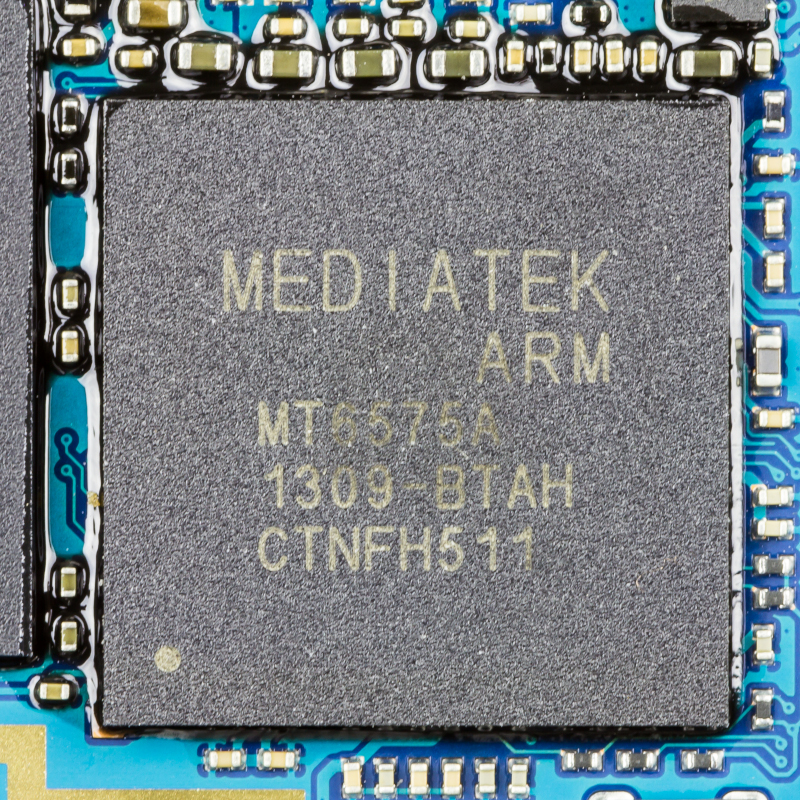
\includegraphics[width=.9\linewidth]{01-grundlagen/img/ARM-Cortex}

        \column{.8\textwidth}
        \begin{block}{System-on-a-Chip}
            \parbox{\linewidth}{
                \smallskip

                Wie ein Microcontroller nur mit einem \textbf{viel leistungsstärkeren
                Rechenkern}, dessen Performance mit dedizierten CPUs vergleichbar ist.
                \textbf{Externer RAM und ROM} werden wie bei einer diskreten CPU über
                ein Speicherinterface angebunden. Darüber hinaus werden oft auch
                \textbf{komplexe Komponenten} wie GPUs, WiFi, Bluetooth, HDMI, etc.
                auf demselben Chip untergebracht.
            }

            \smallskip

            \textbf{Beispiele}: ARM Cortex, AMD AU1000, …
        \end{block}
    \end{columns}
\end{frame}

}

%%% Folie
{
\footnotesize

\begin{frame}{Typischer Systemaufbau eingebetteter Systeme}
    \begin{columns}
        \column{\dimexpr\paperwidth}
        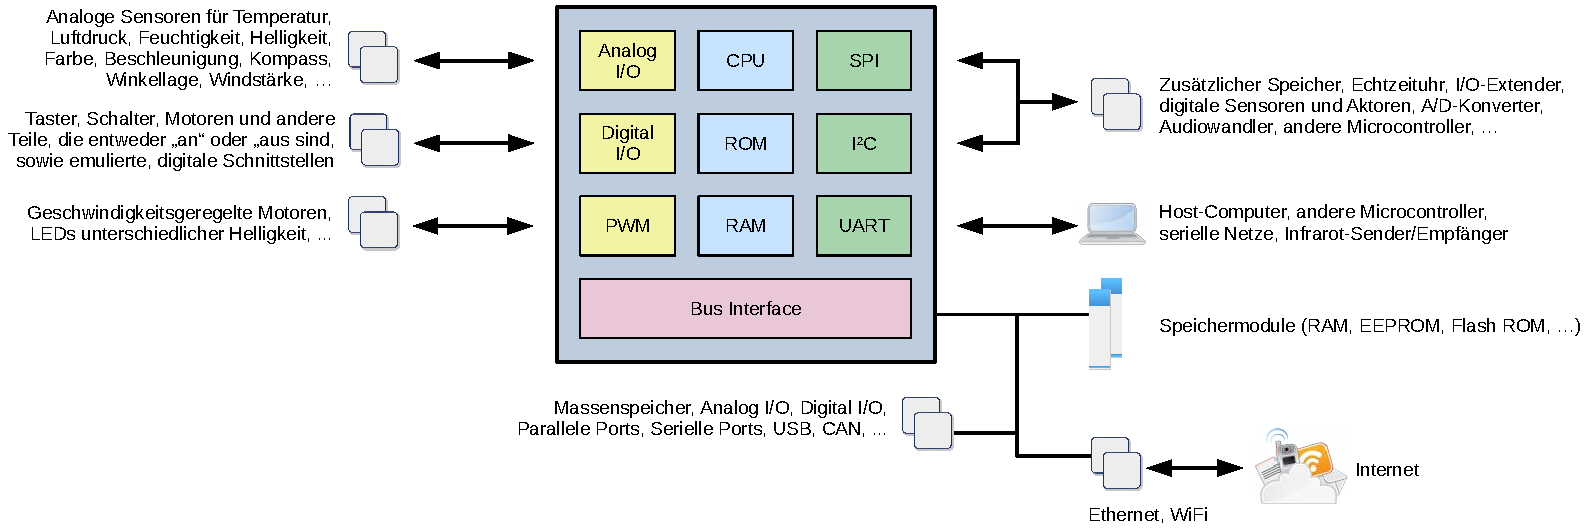
\includegraphics[width=\paperwidth]{01-grundlagen/img/mc_aufbau}
    \end{columns}

    \bigskip

    \begin{columns}
        \begin{column}[T]{.5\textwidth}
            \textbf{Durchschnittlicher Microcontroller}
            \begin{itemize}
                \item 16 MHz Taktgeschwindigkeit
                \item 8 Bit Wortbreite
                \item 32 kB Programmspeicher
                \item 2 kB Hauptspeicher
                \item 14 General Purpose I/Os
                \item Kein Betriebssystem
            \end{itemize}
        \end{column}
        \begin{column}[T]{.5\textwidth}
            \textbf{Durchschnittlicher System-on-a-Chip}
            \begin{itemize}
                \item $\geq$ 200 MHz Taktgeschwindigkeit
                \item $\geq$ 32 Bit Wortbreite
                \item $\geq$ 512 MB Flash ROM
                \item $\geq$ 16 MB Hauptspeicher
                \item $\geq$ 30 General Purpose I/Os
                \item Mit oder ohne Betriebssystem
            \end{itemize}
        \end{column}
    \end{columns}
\end{frame}
}

%%% Folie
\begin{frame}[allowframebreaks]{Fallbeispiel: Yamaha SPX90 (1985)}
    \begin{center}
        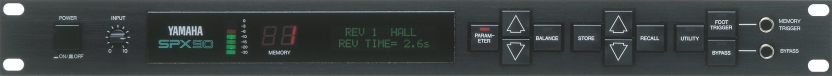
\includegraphics[width=\textwidth]{01-grundlagen/img/spx90-foto}
    \end{center}

    \smallskip

    \begin{itemize}
        \item Frühes, digitales Audio-Effektgerät für professionelle Anwendungen
        \item Hardwareaufbau zweigeteilt in eine Analog- und eine Digitalsektion
        \item \textbf{Analogsektion:} A/D-Wandlung und D/A-Wandlung der Audiosignale
        \item \textbf{Digitalsektion:} Diskret aufgebautes, eingebettetes Computersystem
    \end{itemize}

    \smallskip

    \begin{columns}
        \column[b]{.5\textwidth}
        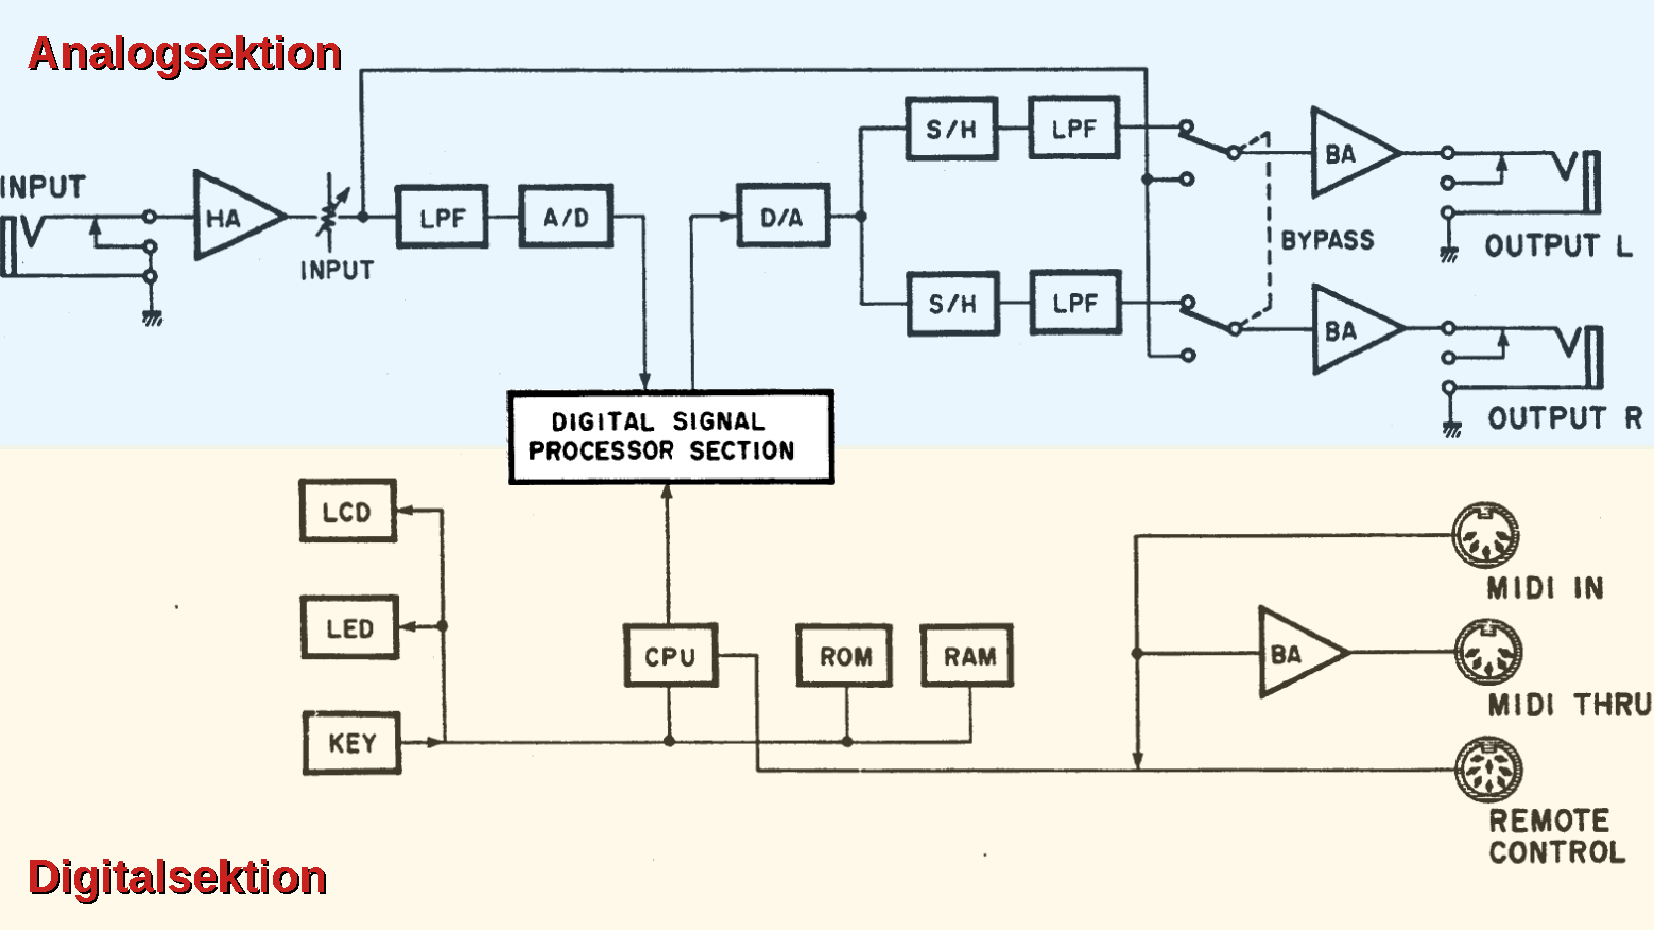
\includegraphics[width=\textwidth]{01-grundlagen/img/spx90-schaltplan-1}

        \column[b]{.5\textwidth}
        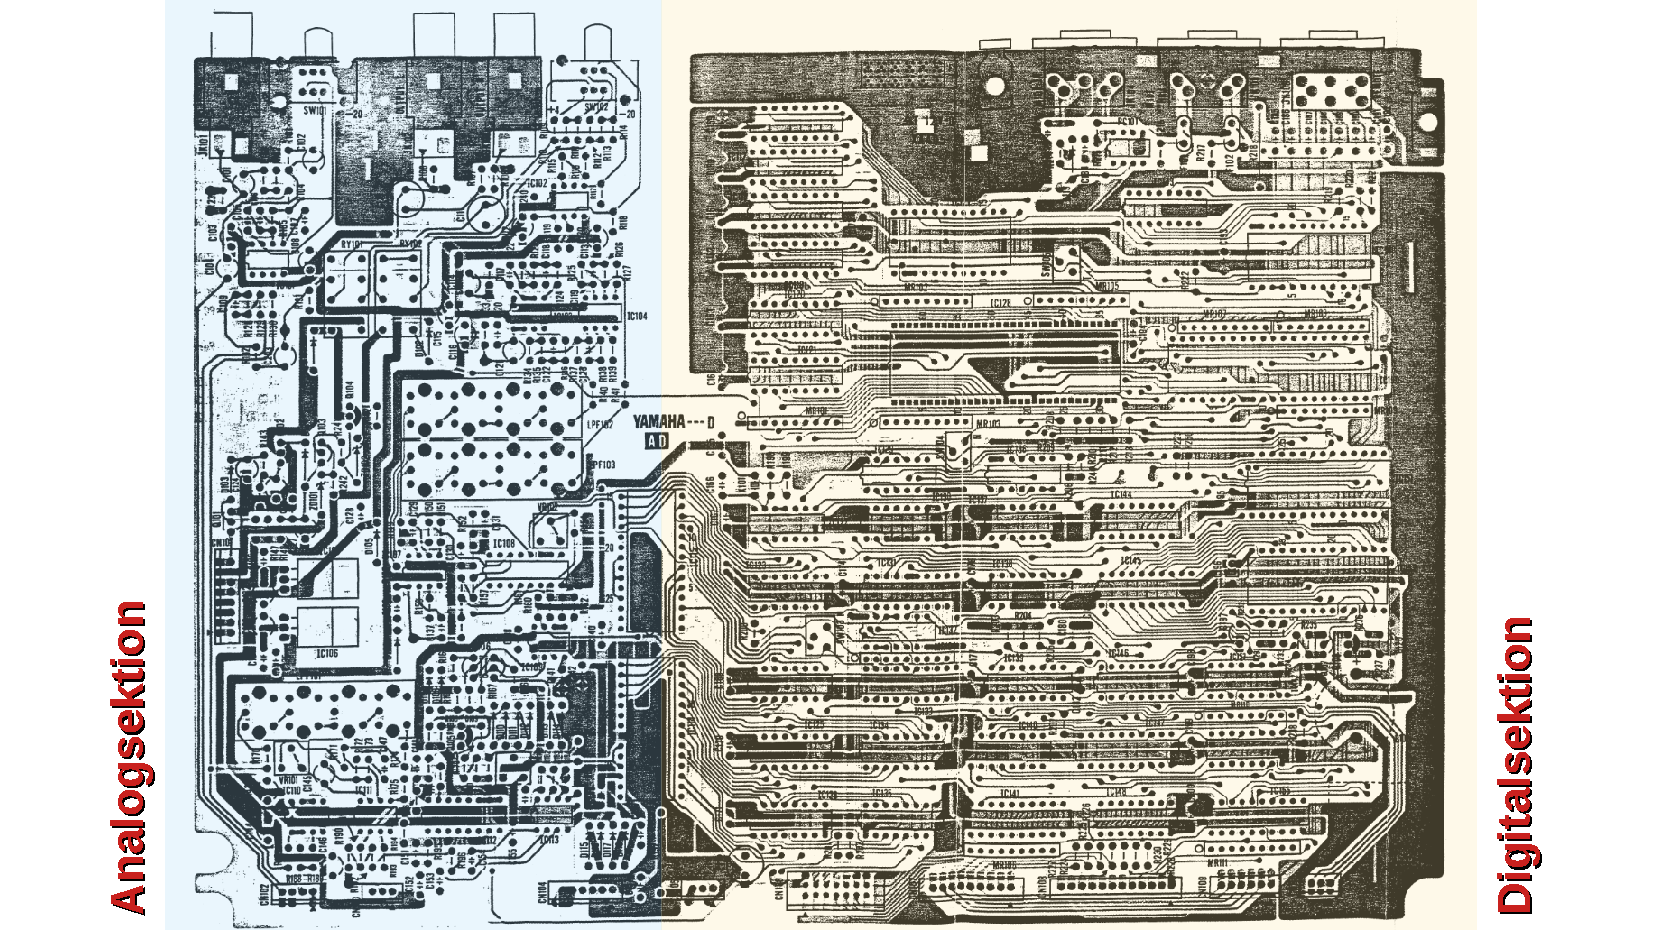
\includegraphics[width=\textwidth]{01-grundlagen/img/spx90-schaltplan-2}
    \end{columns}

    \bigskip

    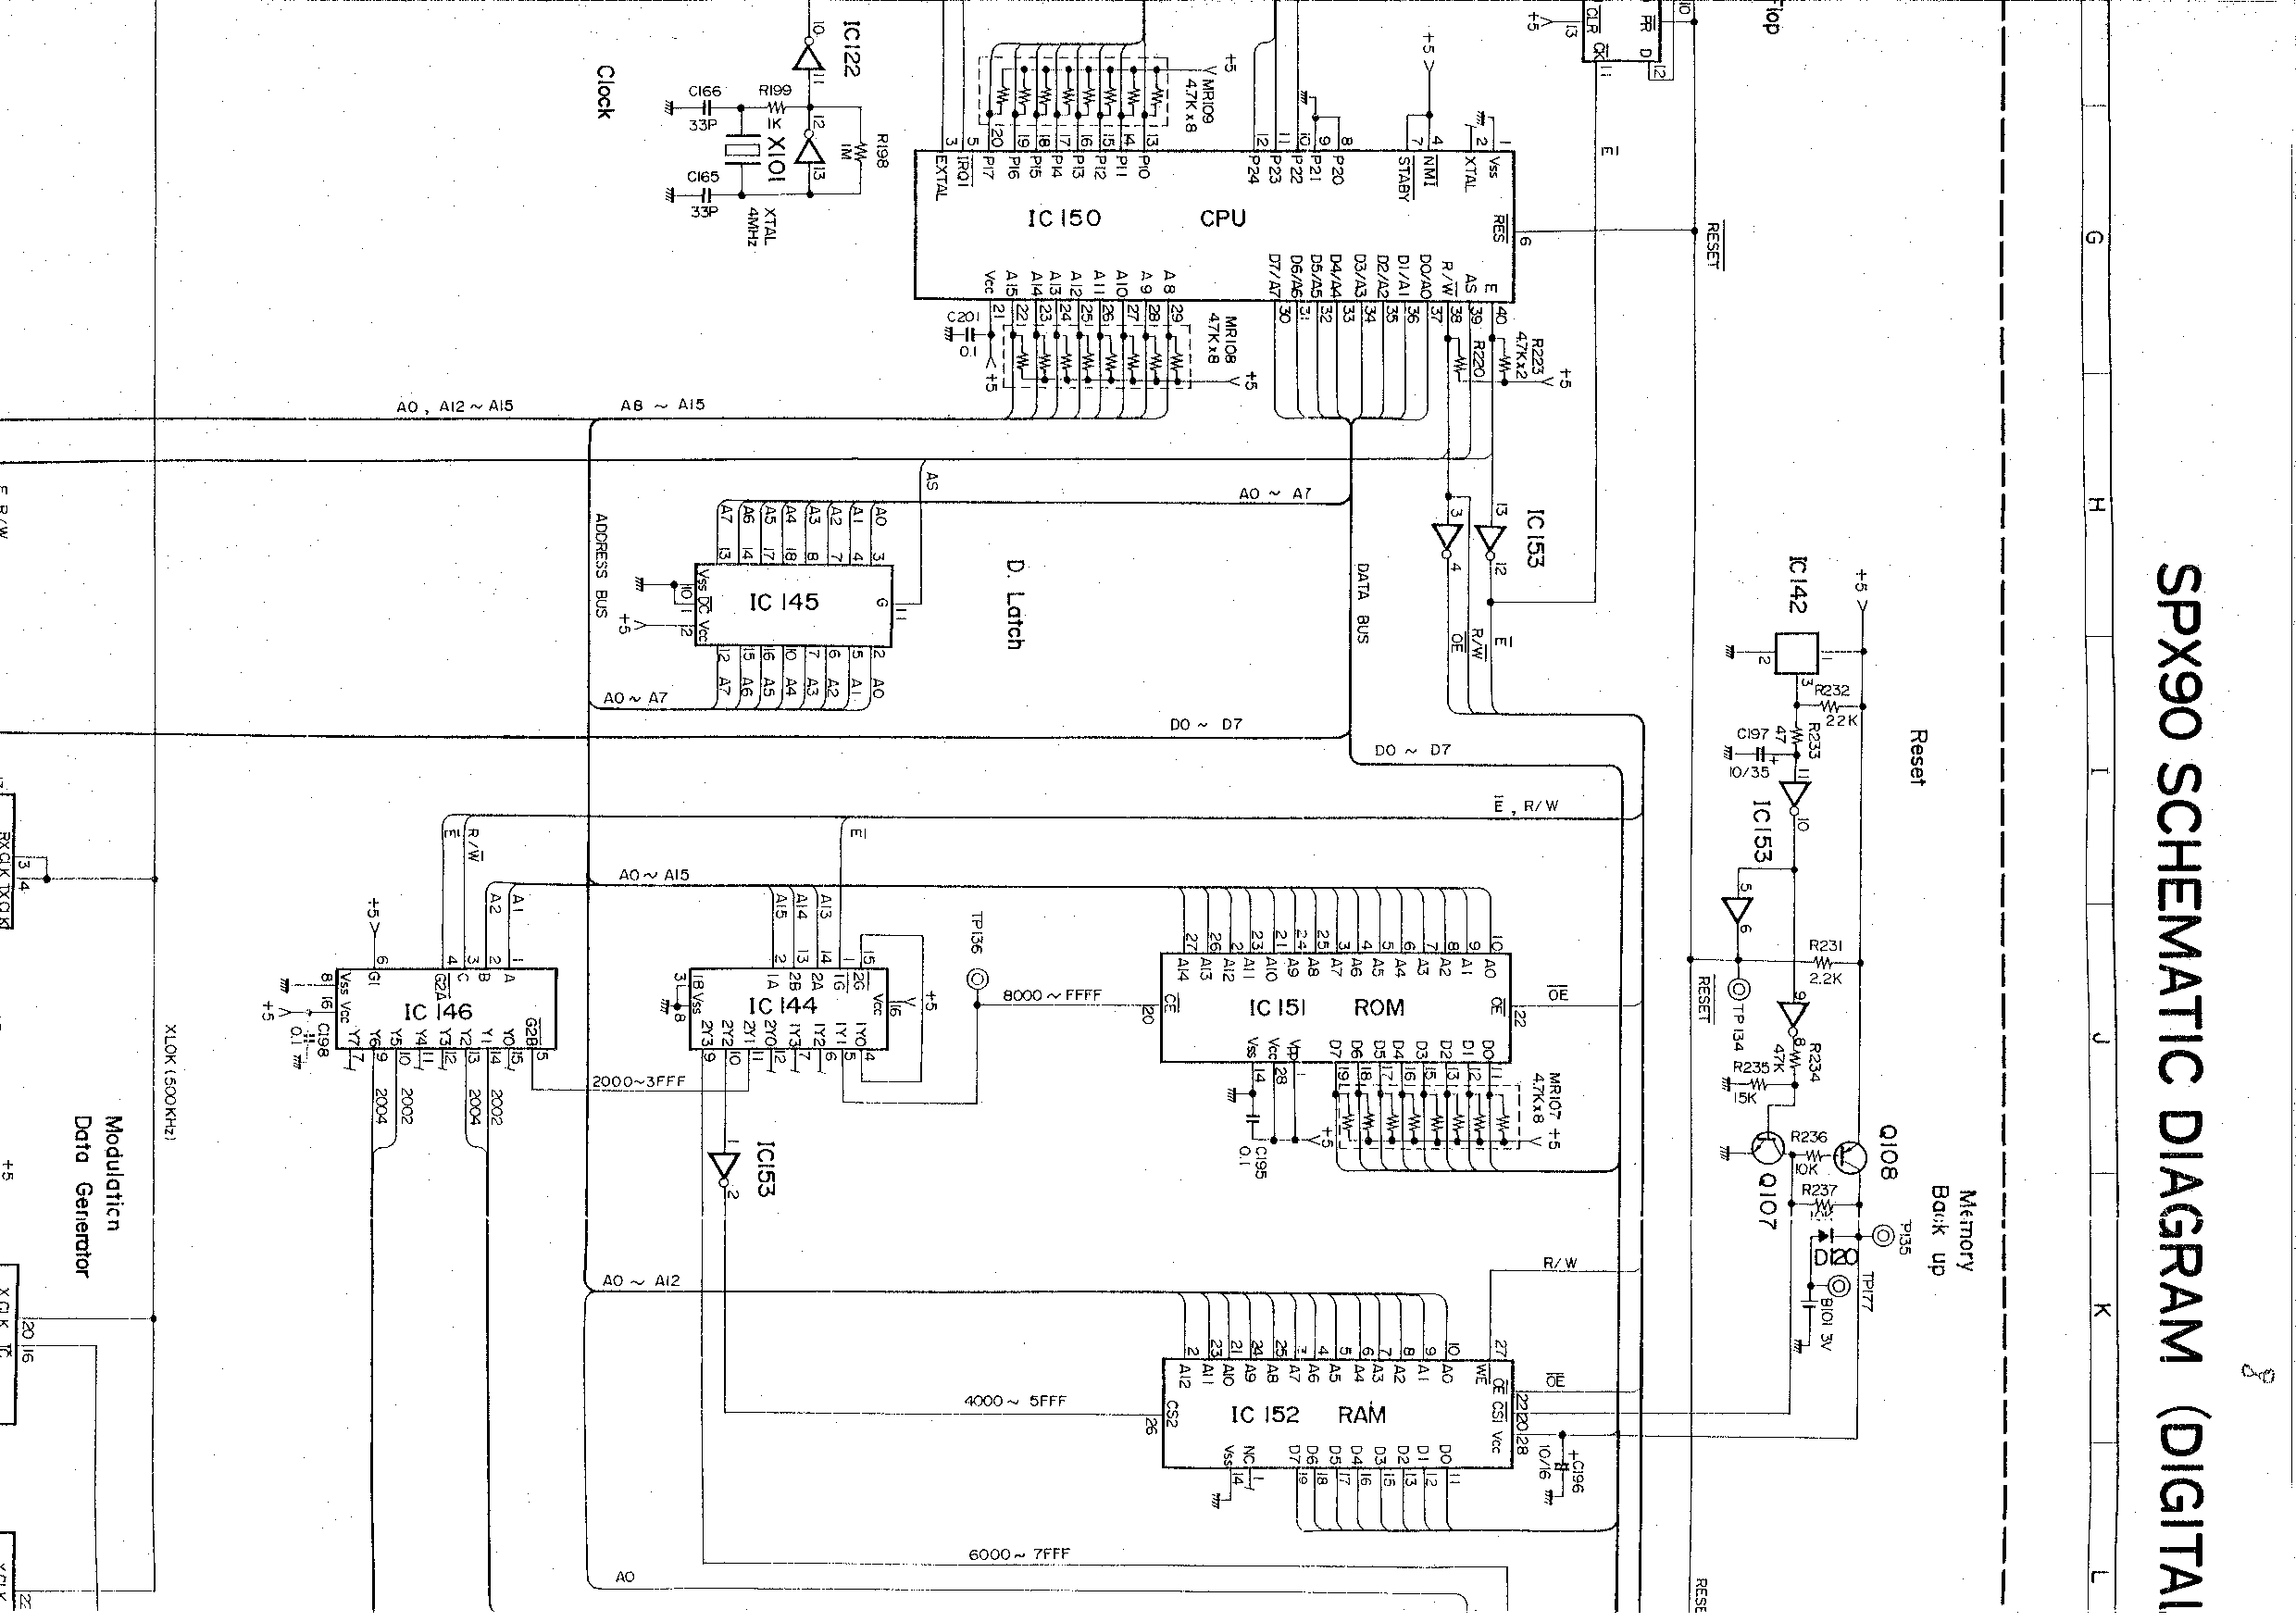
\includegraphics[width=\textwidth]{01-grundlagen/img/spx90-cpuboard}
\end{frame}

%%% Folie
\begin{frame}{Fallbeispiel: IoT-Device mit Sensoren und Aktoren}
    \parbox{\linewidth}{
        \footnotesize
        Die Abbildung zeigt den prototypischen Aufbau eines IoT-Devices mit
        verschiedenen Sensoren und Aktoren. Haupteinheit ist ein Raspberry Pi,
        der über das Flachbandkabel am rechten Rand angeschlossen wird. Der
        Raspberry Pi basiert dabei auf einem System-on-a-Chip, der ein komplettes
        Computersystem in einem einzigen Microchip darstellt.

        \smallskip

        In der Projektentwicklung müssen wir uns meist nur insoweit mit dem
        Hardwareaufbau beschäftigen, wie dies zur Integration der gewünschten
        Sensoren und Aktoren notwendig ist. Eine besondere Herausforderung bleibt
        dabei aber, wie der Prototyp in eine dauerhafte Form überführt werden kann.
    }

    \bigskip

    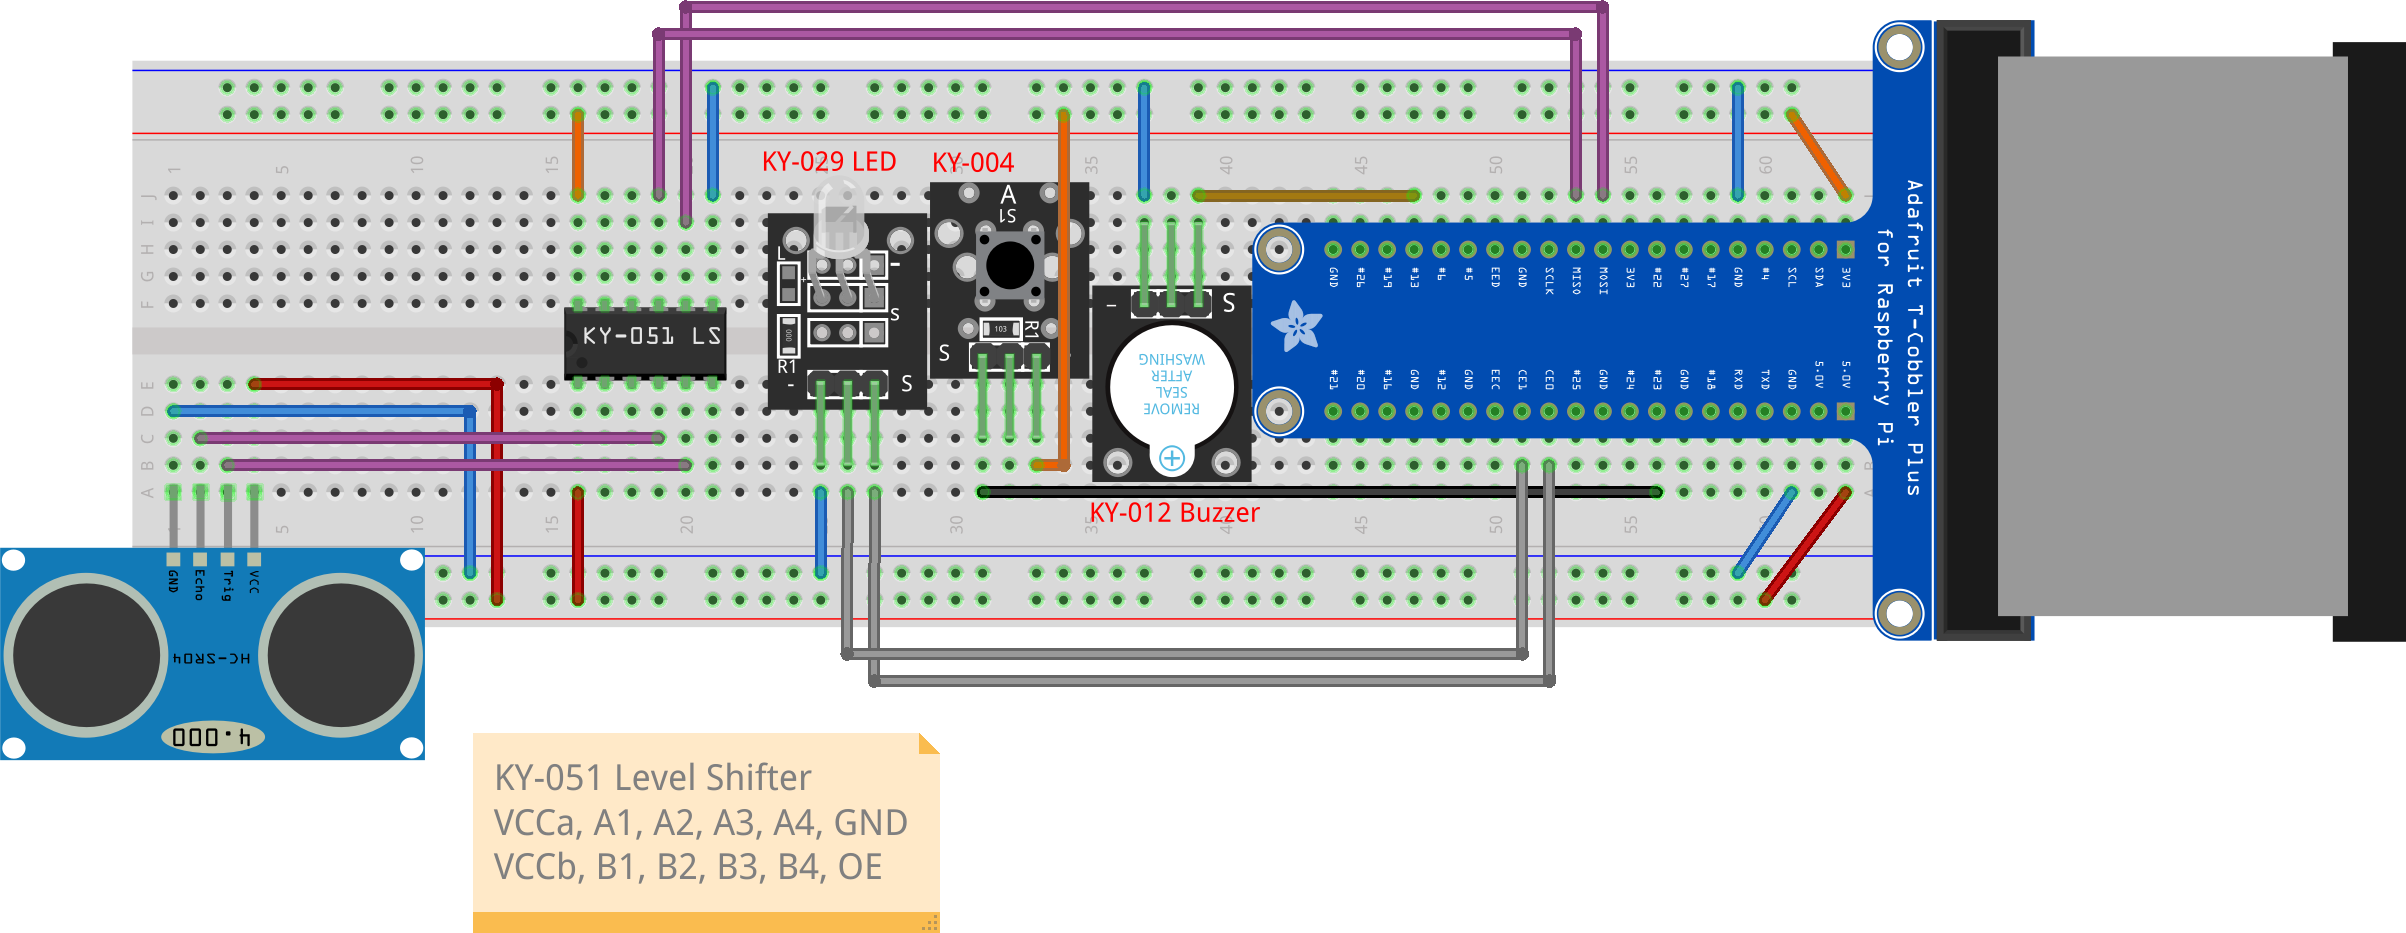
\includegraphics[width=\textwidth]{01-grundlagen/img/einparkhilfe_bb}
\end{frame}

%%% Folie
\begin{frame}[fragile]{Programmierung: Low Level}
    \parbox{\linewidth}{
        \footnotesize
        Dass die Architektur \textbf{diskret aufgebauter, eingebetteter Systeme}
        im Grunde genommen die gleiche wie bei \textbf{Microcontroller/SoC-basierten}
        Systemen ist, zeigt sich auch an den Gemeinsamkeiten der hardwarenahen
        Low-Level-Programmierung (hier am Beispiel für AVR).
    }

    \bigskip

    \begin{lstlisting}[language=C, gobble=8]
        #include <avr/io.h>

        int main(void) {
            PORTD |= (1 << PD2);                    // Pull-Up-Widerstand aktivieren
            DDRB = 0xff;                            // Alle Ausgänge an Port B ausschalten

            while (1) {
                if (bit_is_clear(PIND, PD2)) {      // Pin 2 von Port D auf Ground gezogen?
                    PORTB |= 0b10000000;            // Pin 1 von Port B einschalten
                } else {
                    PORTB &= 0b01111111;            // Pin 1 von Port B ausschalten
                }
            }

            return 0;
        }
    \end{lstlisting}

    \bigskip

    \parbox{\linewidth}{
        \footnotesize
        Für ARM System-on-a-Chip, wie sie im Rasbperry Pi und vielen anderen Geräten
        genutzt werden, sieht der Code ähnlich aus. Das Geheimnis ist, den richtigen
        Wert an die richtige Speicherstelle zu schreiben, um die Hardware zu steuern.
    }
\end{frame}

%%% Folie
\begin{frame}[fragile]{Programmierung: High Level}
    \parbox{\linewidth}{
        \footnotesize
        Aus Gründen der schnelleren und einfacheren Entwicklung sowie der besseren
        Portabilität empfiehlt es sich, zumindest ein einfaches Betriebssystem zu
        nutzen und auf einem höheren Abstraktionsniveu zu programmieren, wenn die
        Systemleistung es zulässt (hier am Beispiel von Python für den Raspberry Pi).
    }

    \smallskip

    \begin{lstlisting}[language=Python, gobble=8, basicstyle=\tiny\ttfamily]
        import os, time
        import RPi.GPIO as GPIO

        GPIO_BUTTON, GPIO_LED = 22, 21

        def on_button_event(button):
            if GPIO.input(button) == GPIO.HIGH:
                GPIO.output(GPIO_LED, True)
            else:
                GPIO.output(GPIO_LED, False)

        if __name__ == "__main__":
            try:
                GPIO.setmode(GPIO.BCM)
                GPIO.setup(GPIO_BUTTON, GPIO.IN, pull_up_down=GPIO.PUD_UP)
                GPIO.setup(GPIO_LED, GPIO.OUT)

                GPIO.add_event_detect(GPIO_BUTTON, GPIO.BOTH)
                GPIO.add_event_callback(GPIO_BUTTON, on_button_event)

                while True:
                    time.sleep(10)
            except KeyboardInterrupt:
                pass

            GPIO.cleanup()
    \end{lstlisting}
\end{frame}

%%% Folie
\begin{frame}{Was nutzen wir in der Vorlesung?}
    \begin{center}
        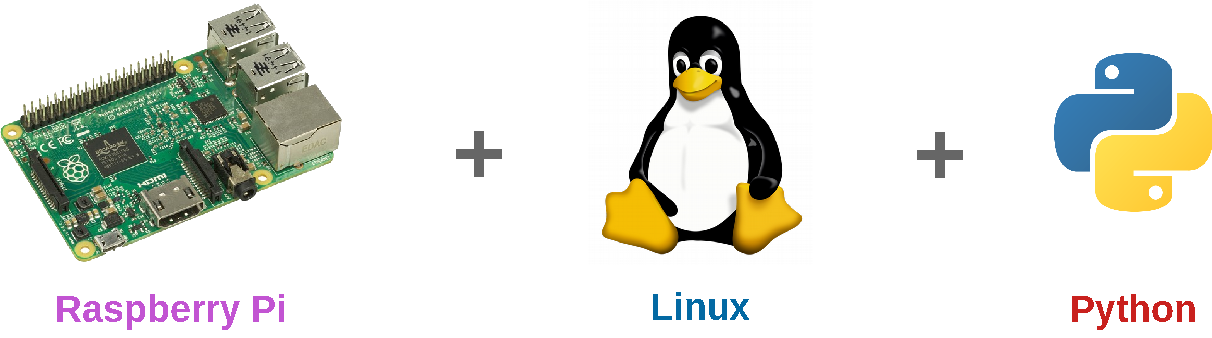
\includegraphics[width=\textwidth]{01-grundlagen/img/raspi-linux-python}
    \end{center}

    \bigskip

    \parbox{\linewidth}{
        \footnotesize
        Wir nutzen eine Kombination aus \textbf{Raspberry Pi}, \textbf{Linux} und
        \textbf{Python}. Sie ist leistungsstark, leicht zu lernen und in der
        IoT-Entwicklung weit verbreitet.

        \medskip

        \begin{itemize}
            \item \textbf{Rasbperry Pi:} Bietet eine vergleichbare Performance wie
            ein älterer Desktopcomputer.

            \item \textbf{Linux:} Beim mitgelieferten Raspberry Pi OS handelt es
            sich um ein angepasstes Debian-Linux. Die meisten Besonderheiten
            eingebetteter Systeme bleiben verborgen, so dass es fast wie ein
            Desktopsystem nutzbar ist.

            \item \textbf{Python:} Ist eine einsteigerfreundliche Programmiersprache
            mit verschiedenen Anwendungsgebieten. Das Pi in Raspberry Pi stand
            deshalb ursprünglich für \glqq{}Python Interpreter\grqq{}.
        \end{itemize}
    }
\end{frame}


%%%%% Folie
%%{
%%    \setbeamertemplate{background canvas}{
%%        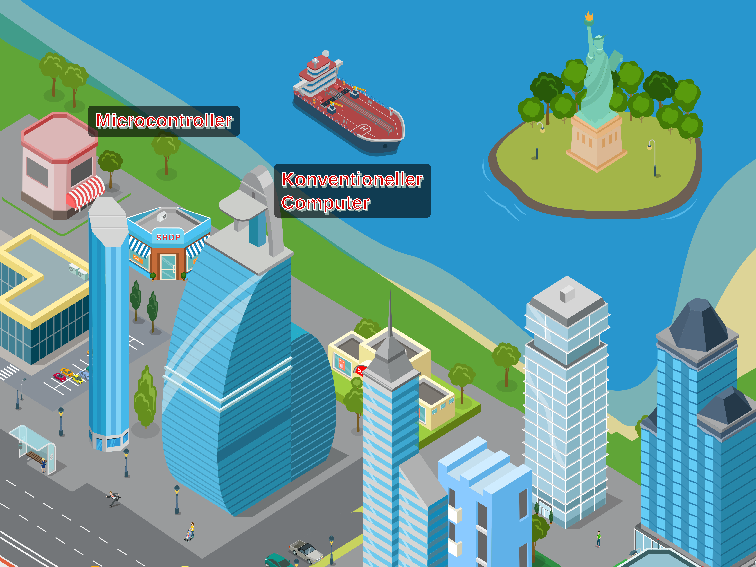
\includegraphics[height=\paperheight, width=\paperwidth]{01-grundlagen/img/software-abstraktion1}
%%    }
%%
%%    \begin{frame}[plain]
%%        \transdissolve
%%
%%        \only<beamer:2|handout:0>{
%%            \transdissolve
%%
%%            \begin{tikzpicture}[remember picture,overlay]
%%                \node at (5.4cm,-0.97cm){
%%                    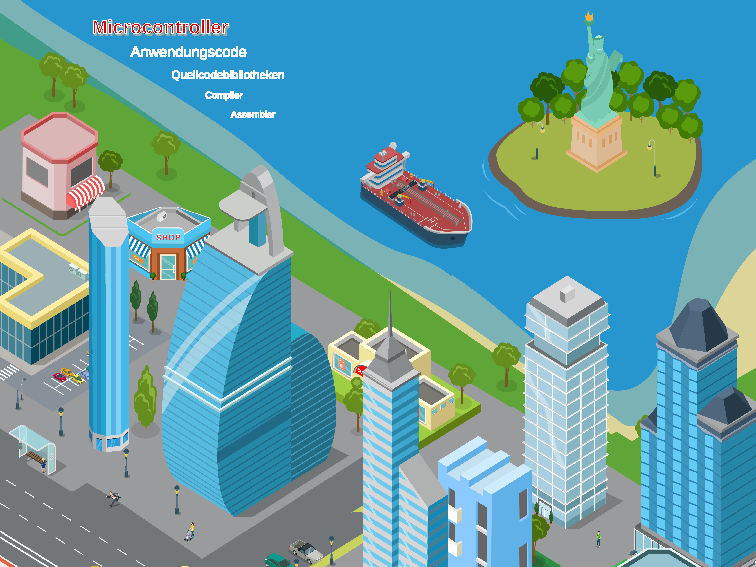
\includegraphics[height=\paperheight, width=\paperwidth]{01-grundlagen/img/software-abstraktion2}
%%                };
%%            \end{tikzpicture}
%%        }
%%
%%        \only<beamer:3|handout:0>{
%%            \transdissolve
%%
%%            \begin{tikzpicture}[remember picture,overlay]
%%                \node at (5.4cm,-0.97cm){
%%                    \includegraphics[height=\paperheight, width=\paperwidth]{01-grundlagen/img/software-abstraktion3}
%%                };
%%            \end{tikzpicture}
%%        }
%%    \end{frame}
%%}{
%%    \setbeamertemplate{background canvas}{
%%        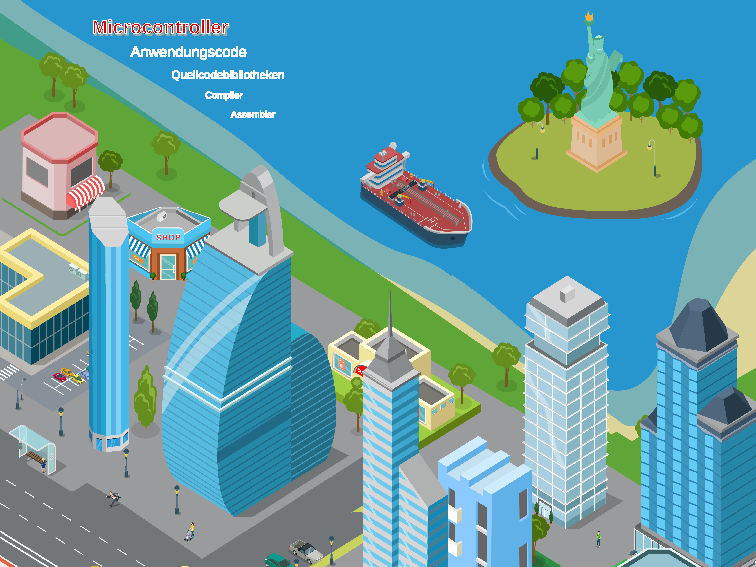
\includegraphics[height=\paperheight, width=\paperwidth]{01-grundlagen/img/software-abstraktion2}
%%    }
%%
%%    \begin{frame}<handout>[plain]
%%        \transdissolve
%%    \end{frame}
%%}{
%%    \setbeamertemplate{background canvas}{
%%        \includegraphics[height=\paperheight, width=\paperwidth]{01-grundlagen/img/software-abstraktion3}
%%    }
%%
%%    \begin{frame}<handout>[plain]
%%        \transdissolve
%%    \end{frame}
%%}
%%
%%%%% Folie
%%\begin{frame}{Softwareseitige Systemanforderungen}
%%    \begin{columns}
%%        \column[T]{.5\textwidth}
%%        \begin{itemize}
%%            \item Sparsamer Umgang mit besonders knappen Ressourcen
%%            \item Verwendung spezialisierter Hardwarekomponenten
%%            \item Störungsfreier Betrieb über sehr lange Zeiträume
%%            \item Firmware-Upgrade ,,over the air''
%%        \end{itemize}
%%
%%        \column[T]{.5\textwidth}
%%        \begin{itemize}
%%            \item Vollständig deterministisches Systemverhalten
%%            \item Oftmals daher nur begrenztes Multi-Tasking
%%            \item Harte, weiche oder eventuelle Echtzeitanforderungen
%%            \item Ausschalten des Geräts ohne ,,Herunterfahren''
%%        \end{itemize}
%%    \end{columns}
%%
%%    \parbox{\linewidth}{
%%        \bigskip
%%        Zur Erfüllung dieser Anforderungen kommen in der Regel angepasste und
%%        besonders schlanke, eingebettete Betriebssysteme zum Einsatz, falls
%%        überhaupt ein Betriebssystem vorhanden ist. Hierbei kann es sich entweder
%%        um speziell für diesen Zweck entwickelte Betriebssysteme wie FreeRTOS
%%        und ITRON oder um eine angepasste Variante größerer Betriebssysteme wie
%%        Linux handeln. Linux bietet sich aufgrund seiner Quelloffenheit und
%%        leichten Portierbarkeit besonders an und wird daher auch entsprechend
%%        oft genutzt.
%%    }
%%\end{frame}
